% Report v2 chapter delivery: Sections 2, 3, 4 and Appendix C.
% Section 1 and Section 5 are intentionally outside this delivery.
% Compile report.tex twice from this directory.
\documentclass[11pt,a4paper]{article}

\usepackage[utf8]{inputenc}
\usepackage[T1]{fontenc}
\usepackage{amsmath, amssymb, amsthm}
\usepackage{geometry}
\geometry{a4paper, margin=2.5cm}
\usepackage{graphicx}
\graphicspath{{figures/}}
\usepackage{booktabs}
\usepackage{longtable}
\usepackage{listings}
\usepackage{xcolor}
\usepackage{hyperref}
\usepackage{xurl}
\newcommand{\field}[1]{\mbox{\texttt{\detokenize{#1}}}}
\usepackage{enumitem}
\usepackage{float}
\usepackage{caption}
\usepackage{subcaption}
\usepackage{bm}
\usepackage{algorithm}
\usepackage{algpseudocode}
\usepackage{mdframed}

% --- colors ---
\definecolor{lecture}{RGB}{70,130,180}
\definecolor{seminar}{RGB}{205,92,92}
\definecolor{formbg}{RGB}{250,250,245}
\definecolor{formframe}{RGB}{180,170,140}

% --- code listing style (Python) ---
\lstset{
    language=Python,
    basicstyle=\ttfamily\scriptsize,
    keywordstyle=\color{blue}\bfseries,
    commentstyle=\color{green!40!black},
    stringstyle=\color{red!70!black},
    numbers=left,
    numberstyle=\tiny\color{gray},
    frame=single,
    breaklines=true,
    showstringspaces=false,
    tabsize=4,
    captionpos=b,
}

% --- theorem-like environments (course-level set) ---
\newtheorem{theorem}{Theorem}[section]
\newtheorem{lemma}[theorem]{Lemma}
\newtheorem{proposition}[theorem]{Proposition}
\newtheorem{corollary}[theorem]{Corollary}
\theoremstyle{definition}
\newtheorem{definition}[theorem]{Definition}
\newtheorem{assumption}[theorem]{Assumption}
\newtheorem{example}[theorem]{Example}
\theoremstyle{remark}
\newtheorem{remark}[theorem]{Remark}

% --- algorithm style ---
\algrenewcommand{\algorithmicrequire}{\textbf{Input:}}
\algrenewcommand{\algorithmicensure}{\textbf{Output:}}
\algrenewcommand{\algorithmiccomment}[1]{\hfill\textcolor{gray}{\# #1}}

% --- form box (for appendices) ---
\newmdenv[
    backgroundcolor=formbg,
    linecolor=formframe,
    linewidth=0.8pt,
    roundcorner=3pt,
    innermargin=5pt,
    outermargin=5pt,
    innertopmargin=8pt,
    innerbottommargin=8pt
]{formbox}


\title{\textbf{Numerical Integration of the Polar-Factor Gradient Flow}\\[2mm]
\large Report v2: Sections 2--4 and Appendix C}
\author{}
\date{28 September 2026}
\begin{document}
\maketitle
\begingroup\small
\tableofcontents
\endgroup
\newpage
\setcounter{section}{1}
\section{Discretisation and Analysis}
% ============================================================

\subsection{Discrete Schemes}
\label{sec:discrete_schemes}

We consider a general initial value problem (IVP), which may be non-autonomous, on the compact temporal interval $t \in [t_0, T]$:
\begin{equation}
\label{eq:general_ivp}
\dot{\mathbf{y}}(t) = \mathbf{f}(t, \mathbf{y}(t)), \quad \mathbf{y}(t_0) = \mathbf{y}_0 \in \mathbb{R}^d,
\end{equation}
where $\mathbf{f}: [t_0, T] \times \mathbb{R}^d \to \mathbb{R}^d$ is assumed to be sufficiently smooth and locally Lipschitz continuous with respect to $\mathbf{y}$. Let the continuous interval $[t_0, T]$ be partitioned by a uniform grid
$t_n=t_0+nh$, $n=0,1,\ldots,N$, where $h=(T-t_0)/N>0$. Integrating \eqref{eq:general_ivp} over a single time step $[t_n,t_{n+1}]$ yields the exact Volterra integral relation:
\begin{equation}
\label{eq:integral_form}
\mathbf{y}(t_{n+1}) - \mathbf{y}(t_n) = \int_{t_n}^{t_{n+1}} \mathbf{f}(t, \mathbf{y}(t)) \, \mathrm{d}t.
\end{equation}
Different numerical approximations of the quadrature in \eqref{eq:integral_form} give rise to distinct numerical schemes with contrasting orders of accuracy, computational costs, and stability domains.

For Topic~5, the state is a square matrix
$\mathbf{X}(t)\in\mathbb{R}^{n\times n}$ satisfying the autonomous
matrix differential equation
\begin{equation}
\label{eq:topic5_matrix_model}
\dot{\mathbf{X}}(t)
=
\mathbf{f}(\mathbf{X}(t))
=
\mathbf{X}(t)\left(\mathbf{I}_n-\mathbf{X}(t)^T\mathbf{X}(t)\right),
\qquad
\mathbf{X}(0)=\mathbf{X}_0.
\end{equation}
When vectorised in column-major order,
$\mathbf{y}=\operatorname{vec}(\mathbf{X})\in\mathbb{R}^{n^2}$,
this becomes the standard vector-valued IVP \eqref{eq:general_ivp}; the
matrix formulas below are therefore equivalent to the vector formulation.
The polar-factor interpretation follows the convention in \cite{higham1986}. This evolution is the ambient Euclidean negative-gradient flow of
$\Phi(\mathbf X)=\|\mathbf X^T\mathbf X-\mathbf I_n\|_F^2/4$.
For a separate differentiable objective $g$ constrained to the
orthogonal group, let $\mathbf G=\nabla g(\mathbf X)$ and
$\mathbf X^T\mathbf X=\mathbf I_n$. Its tangent projection is
\begin{equation}
\label{eq:orthogonal_tangent_projection}
P_{\mathbf X}(\mathbf G)
=\mathbf G-\mathbf X\operatorname{sym}(\mathbf X^T\mathbf G)
=\mathbf X\operatorname{skew}(\mathbf X^T\mathbf G),
\end{equation}
where $\operatorname{sym}(A)=(A+A^T)/2$ and
$\operatorname{skew}(A)=(A-A^T)/2$; the corresponding constrained
gradient flow is $\dot{\mathbf X}=-P_{\mathbf X}(\mathbf G)$.
The expression $(\mathbf I_n-\mathbf X\mathbf X^T)\mathbf G$ vanishes
for every square orthogonal $\mathbf X$ and is not this tangent
projection. This distinction is relevant because every orthogonal
matrix is an equilibrium of the ambient flow \eqref{eq:topic5_matrix_model}.

\subsubsection{Explicit Euler Method}
The simplest one-step method is obtained by approximating the integral in \eqref{eq:integral_form} via the left-hand rectangle quadrature rule, evaluating the integrand solely at the known base state $(t_n, \mathbf{y}(t_n))$:
\begin{equation}
\label{eq:explicit_euler}
\mathbf{y}_{n+1} = \mathbf{y}_n + h \mathbf{f}(t_n, \mathbf{y}_n).
\end{equation}
Equation \eqref{eq:explicit_euler} is strictly explicit; advancing the state from $t_n$ to $t_{n+1}$ incurs exactly one evaluation of the vector field $\mathbf{f}$ without requiring any linear or nonlinear system solves. Its cost is therefore one right-hand-side evaluation per step; the floating-point cost depends on the structure of $\mathbf{f}$ (for the matrix flow considered below, the dominant matrix products cost $\mathcal{O}(n^3)$). The method is conditionally stable and imposes severe step-size restrictions when applied to stiff ODE systems.

For the Topic~5 matrix flow \eqref{eq:topic5_matrix_model}, the
Explicit Euler update is
\begin{equation}
\label{eq:topic5_explicit_euler}
\mathbf{X}_{n+1}
=
\mathbf{X}_n
+h\,\mathbf{X}_n
\left(\mathbf{I}_n-\mathbf{X}_n^T\mathbf{X}_n\right).
\end{equation}

\subsubsection{Classical Fourth-Order Runge--Kutta Method (RK4)}
To achieve higher-order accuracy without computing higher-order analytical derivatives of $\mathbf{f}$, the classical fourth-order Runge--Kutta scheme (RK4) evaluates the continuous vector field at four intermediate stages across $[t_n, t_{n+1}]$:
\begin{align}
\mathbf{k}_1 &= \mathbf{f}(t_n, \mathbf{y}_n), \label{eq:rk4_k1} \\
\mathbf{k}_2 &= \mathbf{f}\left(t_n + \frac{h}{2}, \mathbf{y}_n + \frac{h}{2}\mathbf{k}_1\right), \label{eq:rk4_k2} \\
\mathbf{k}_3 &= \mathbf{f}\left(t_n + \frac{h}{2}, \mathbf{y}_n + \frac{h}{2}\mathbf{k}_2\right), \label{eq:rk4_k3} \\
\mathbf{k}_4 &= \mathbf{f}(t_n + h, \mathbf{y}_n + h\mathbf{k}_3), \label{eq:rk4_k4}
\end{align}
and synthesizes them with the classical RK4 weights:
\begin{equation}
\label{eq:rk4_update}
\mathbf{y}_{n+1} = \mathbf{y}_n + \frac{h}{6} \left(\mathbf{k}_1 + 2\mathbf{k}_2 + 2\mathbf{k}_3 + \mathbf{k}_4\right).
\end{equation}
The algebraic structure of any $s$-stage Runge--Kutta method can be compactly encapsulated by its Butcher tableau:
\begin{equation}
\label{eq:butcher_general}
\begin{array}{c|c}
\mathbf{c} & \mathbf{A} \\
\hline
& \mathbf{b}^T
\end{array}
\end{equation}

For the matrix vector field
$\mathbf{f}(\mathbf{X})=\mathbf{X}(\mathbf{I}_n-\mathbf{X}^T\mathbf{X})$,
the RK4 stages are evaluated with matrix arithmetic:
\begin{align}
\mathbf{K}_1
&=\mathbf{f}(\mathbf{X}_n), \label{eq:topic5_rk4_k1}\\
\mathbf{K}_2
&=\mathbf{f}\left(\mathbf{X}_n+\frac{h}{2}\mathbf{K}_1\right), \label{eq:topic5_rk4_k2}\\
\mathbf{K}_3
&=\mathbf{f}\left(\mathbf{X}_n+\frac{h}{2}\mathbf{K}_2\right), \label{eq:topic5_rk4_k3}\\
\mathbf{K}_4
&=\mathbf{f}\left(\mathbf{X}_n+h\mathbf{K}_3\right). \label{eq:topic5_rk4_k4}
\end{align}
The corresponding matrix update is
\begin{equation}
\label{eq:topic5_rk4_update}
\mathbf{X}_{n+1}
=\mathbf{X}_n+\frac{h}{6}
\left(\mathbf{K}_1+2\mathbf{K}_2+2\mathbf{K}_3+\mathbf{K}_4\right).
\end{equation}
For the classical RK4 method, the standard coefficients $\mathbf{A} \in \mathbb{R}^{4 \times 4}$, $\mathbf{b} \in \mathbb{R}^4$, and $\mathbf{c} \in \mathbb{R}^4$ are:
\begin{equation}
\label{eq:rk4_butcher}
\begin{array}{c|cccc}
0   & 0   & 0   & 0 & 0 \\
1/2 & 1/2 & 0   & 0 & 0 \\
1/2 & 0   & 1/2 & 0 & 0 \\
1   & 0   & 0   & 1 & 0 \\
\hline
    & 1/6 & 1/3 & 1/3 & 1/6
\end{array}
\end{equation}
Because the Runge--Kutta matrix $\mathbf{A}$ in \eqref{eq:rk4_butcher} is strictly lower triangular with a vanishing main diagonal ($a_{ij} = 0$ for all $j \ge i$), each stage derivative $\mathbf{k}_i$ depends solely on the previously evaluated stage vectors $\mathbf{k}_1, \dots, \mathbf{k}_{i-1}$, preserving an explicit computation sequence.

\subsubsection{Implicit Euler Method with Damped Newton Iteration}
When the physical system exhibits stiffness, explicit schemes encounter numerical blow-up unless $h$ is restricted to excessively small time steps. The right-hand rectangle rule gives the Implicit (Backward) Euler scheme:
\begin{equation}
\label{eq:implicit_euler}
\mathbf{y}_{n+1} = \mathbf{y}_n + h \mathbf{f}(t_{n+1}, \mathbf{y}_{n+1}).
\end{equation}
Because the unknown state $\mathbf{y}_{n+1}$ appears nonlinearly within the argument of $\mathbf{f}$, \eqref{eq:implicit_euler} constitutes a coupled system of $d$ nonlinear algebraic equations at each time step.

For Topic~5, the Implicit Euler equation becomes the nonlinear matrix
equation
\begin{equation}
\label{eq:topic5_implicit_euler}
\mathbf{X}_{n+1}
=\mathbf{X}_n+h\,\mathbf{X}_{n+1}
\left(\mathbf{I}_n-\mathbf{X}_{n+1}^T\mathbf{X}_{n+1}\right).
\end{equation}

Let $\mathbf{w} \in \mathbb{R}^d$ represent the unknown state vector at $t_{n+1}$. We define the nonlinear residual mapping $\mathbf{F}: \mathbb{R}^d \to \mathbb{R}^d$ by collecting all terms on one side:
\begin{equation}
\label{eq:newton_residual}
\mathbf{F}(\mathbf{w}) := \mathbf{w} - \mathbf{y}_n - h \mathbf{f}(t_{n+1}, \mathbf{w}) = \mathbf{0}.
\end{equation}
To solve $\mathbf{F}(\mathbf{w}) = \mathbf{0}$ iteratively, we linearize $\mathbf{F}$ around a current trial estimate $\mathbf{w}^{(k)}$ via first-order multivariate Taylor expansion:
\begin{equation}
\label{eq:taylor_residual}
\mathbf{F}\left(\mathbf{w}^{(k)} + \boldsymbol{\delta}^{(k)}\right) \approx \mathbf{F}\left(\mathbf{w}^{(k)}\right) + \mathbf{J}_{\mathbf{F}}\left(\mathbf{w}^{(k)}\right) \boldsymbol{\delta}^{(k)} = \mathbf{0},
\end{equation}
where $\mathbf{J}_{\mathbf{F}}(\mathbf{w}) \in \mathbb{R}^{d \times d}$ is the Fr\'echet derivative (Jacobian matrix) of the residual operator $\mathbf{F}$ with respect to $\mathbf{w}$. Applying the multivariate chain rule to \eqref{eq:newton_residual} yields:
\begin{equation}
\label{eq:residual_jacobian}
\mathbf{J}_{\mathbf{F}}(\mathbf{w}) = \frac{\partial \mathbf{F}}{\partial \mathbf{w}} = \frac{\partial}{\partial \mathbf{w}} \left(\mathbf{w} - \mathbf{y}_n - h \mathbf{f}(t_{n+1}, \mathbf{w})\right) = \mathbf{I}_d - h \mathbf{J}_{\mathbf{f}}(t_{n+1}, \mathbf{w}),
\end{equation}
where $\mathbf{I}_d$ is the $d \times d$ identity matrix and $\mathbf{J}_{\mathbf{f}}(\cdot) = \frac{\partial \mathbf{f}}{\partial \mathbf{y}} \in \mathbb{R}^{d \times d}$ is the analytical Jacobian matrix of the continuous ODE vector field.

For the Topic~5 vector field
$\mathbf{f}(\mathbf{X})=\mathbf{X}(\mathbf{I}_n-\mathbf{X}^T\mathbf{X})$,
the Fr\'echet derivative in a matrix direction
$\mathbf{H}\in\mathbb{R}^{n\times n}$ is
\begin{equation}
\label{eq:topic5_frechet_derivative}
\mathcal{D}\mathbf{f}(\mathbf{X})[\mathbf{H}]
=\mathbf{H}(\mathbf{I}_n-\mathbf{X}^T\mathbf{X})
-\mathbf{X}(\mathbf{H}^T\mathbf{X}+\mathbf{X}^T\mathbf{H}).
\end{equation}
Consequently, if $\mathbf{G}(\mathbf{X})$ denotes the matrix residual of
an Implicit Euler step,
\begin{equation}
\label{eq:topic5_matrix_residual}
\mathbf{G}(\mathbf{X})=\mathbf{X}-\mathbf{X}_n-h\mathbf{f}(\mathbf{X}),
\end{equation}
then
\begin{equation}
\label{eq:topic5_residual_frechet}
\mathcal{D}\mathbf{G}(\mathbf{X})[\mathbf{H}]
=\mathbf{H}-h\,\mathcal{D}\mathbf{f}(\mathbf{X})[\mathbf{H}].
\end{equation}
After column-major vectorisation, this is exactly the residual Jacobian
$\mathbf{I}_{n^2}-h\mathbf{J}_{\mathbf f}(\mathbf X)$ used by Newton's method.

The standard full Newton direction $\boldsymbol{\delta}^{(k)}$ is determined by solving the linear algebraic system:
\begin{equation}
\label{eq:newton_linear_system}
\mathbf{J}_{\mathbf{F}}\left(\mathbf{w}^{(k)}\right) \boldsymbol{\delta}^{(k)} = -\mathbf{F}\left(\mathbf{w}^{(k)}\right).
\end{equation}
In practical stiff and highly nonlinear implementations, the initial state $\mathbf{w}^{(0)} = \mathbf{y}_n$ may fall outside the local quadratic attraction basin, causing standard full Newton iterations ($\mathbf{w}^{(k+1)} = \mathbf{w}^{(k)} + \boldsymbol{\delta}^{(k)}$) to suffer from severe overshoot and divergence. We therefore use a residual-decreasing backtracking line search with damping parameter $\alpha \in (0,1]$:
\begin{equation}
\label{eq:newton_damped_update}
\mathbf{w}^{(k+1)} = \mathbf{w}^{(k)} + \alpha \boldsymbol{\delta}^{(k)}.
\end{equation}
The Newton residual is accepted using the scale-aware criterion
$\|\mathbf{F}(\mathbf{w})\|_\infty\le
\mathrm{atol}_F+\mathrm{rtol}_F\|\mathbf{w}\|_\infty$.
This prevents the stopping rule from depending on the absolute size of
the matrix state alone.
Algorithm~\ref{alg:implicit_euler_newton} describes the Implicit Euler
one-step solve implemented in \texttt{code/solvers.py}. It returns either
the selected root or a failure signal. The outer fixed-grid solver reports
that failure without changing its uniform grid; the adaptive solver rejects
the trial and retries from the last accepted state with half the step.

\begin{algorithm}[htbp]
\caption{One Implicit Euler step with residual-decreasing damped Newton}
\label{alg:implicit_euler_newton}
\footnotesize
\begin{algorithmic}[1]
\Require $t_n,\mathbf y_n,h,\mathbf f,\mathbf J_{\mathbf f}$; tolerance
  $\varepsilon_F$; maximum Newton updates $K_{\max}$.
\Ensure Root $\mathbf w$ satisfying
  $\|\mathbf F(\mathbf w)\|_\infty\leq
  \varepsilon_F(1+\|\mathbf w\|_\infty)$, or failure.
\State $\mathbf w\gets\mathbf y_n$ \Comment{Previous state is the initial guess.}
\For{$k=0,\ldots,K_{\max}$}
    \State $\mathbf F\gets\mathbf w-\mathbf y_n-h\mathbf f(t_n+h,\mathbf w)$
    \If{$\mathbf F$ is non-finite}
        \State \Return failure
    \EndIf
    \If{$\|\mathbf F\|_\infty\leq
            \varepsilon_F(1+\|\mathbf w\|_\infty)$}
        \State \Return $\mathbf w$
    \EndIf
    \If{$k=K_{\max}$}
        \State \Return failure
    \EndIf
    \State $\mathbf J_F\gets\mathbf I_d-h\mathbf J_{\mathbf f}(t_n+h,\mathbf w)$
    \State Solve $\mathbf J_F\boldsymbol\delta=-\mathbf F$;
           if singular, \Return failure
    \State $\alpha\gets1$; accepted $\gets$ false
    \While{$\alpha\geq10^{-4}$}
        \State $\mathbf w_{\rm try}\gets\mathbf w+\alpha\boldsymbol\delta$
        \State $\mathbf F_{\rm try}\gets
          \mathbf w_{\rm try}-\mathbf y_n-h\mathbf f(t_n+h,\mathbf w_{\rm try})$
        \If{$\mathbf F_{\rm try}$ is finite and
            $\|\mathbf F_{\rm try}\|_\infty<\|\mathbf F\|_\infty$}
            \State $\mathbf w\gets\mathbf w_{\rm try}$; accepted $\gets$ true
            \State \textbf{break}
        \EndIf
        \State $\alpha\gets\alpha/2$
    \EndWhile
    \If{not accepted}
        \State \Return failure
    \EndIf
\EndFor
\end{algorithmic}
\end{algorithm}

In our runs $\varepsilon_F=10^{-12}$ and $K_{\max}=20$. The candidate
residual is evaluated at $\mathbf w_{\rm try}$ in \emph{both} occurrences of
the unknown, which is essential for the line search.



\subsection{Consistency and Truncation Error}

\label{sec:consistency_and_truncation_error}

\subsubsection{Theoretical Assumptions and Local Defect}
To rigorously quantify the asymptotic discretization error of the numerical integrators formulated in Section~\ref{sec:discrete_schemes}, we establish the analytical foundation under classical regularity assumptions. Let the continuous vector field $\mathbf{f}: [t_0, T] \times \mathbb{R}^d \to \mathbb{R}^d$ satisfy the following conditions:
\begin{enumerate}
    \item \textbf{Lipschitz Continuity:} There exists a finite Lipschitz constant $L > 0$ such that on a bounded domain $\Omega \subset [t_0, T] \times \mathbb{R}^d$:
    \begin{equation}
    \label{eq:lipschitz_condition}
    \|\mathbf{f}(t, \mathbf{u}) - \mathbf{f}(t, \mathbf{v})\| \le L \|\mathbf{u} - \mathbf{v}\|, \quad \forall (t, \mathbf{u}), (t, \mathbf{v}) \in \Omega.
    \end{equation}
    By the Picard--Lindel\"of theorem, together with continuity in $t$, condition \eqref{eq:lipschitz_condition} guarantees local existence and uniqueness. A solution on the full interval requires that the trajectory remain in a bounded region where these assumptions continue to hold.
    \item \textbf{Sufficient Smoothness:} For the explicit remainders through $\mathcal{O}(h^3)$ in the Euler expansions and $\mathcal{O}(h^6)$ in the RK4 expansion below, assume that $\mathbf f$ has continuous derivatives through order five on a bounded neighbourhood of the solution and that $\mathbf y\in C^6[t_0,T]$. The usual order bounds $\boldsymbol\rho^{\mathrm{Euler}}=\mathcal{O}(h^2)$ and $\boldsymbol\rho^{\mathrm{RK4}}=\mathcal{O}(h^5)$ require fewer derivatives. For Topic~5, $\mathbf f(\mathbf X)=\mathbf X(\mathbf I-\mathbf X^T\mathbf X)$ is polynomial; its exact finite-time solution in \eqref{eq:singular_value_exact} is smooth, including when an initial singular value is zero, so the stronger assumptions used here hold on every finite interval.
\end{enumerate}

Any generic single-step integration scheme advancing from $t_n$ to $t_{n+1}=t_n+h$ can be cast into the increment form:
\begin{equation}
\label{eq:general_increment_function}
\mathbf{y}_{n+1} = \mathbf{y}_n + h \mathbf{\Phi}(t_n, \mathbf{y}_n, h),
\end{equation}
where $\mathbf{\Phi}$ represents the numerical increment function. For Explicit Euler and RK4 it is explicit. For Implicit Euler, define the one-step solution map $\boldsymbol{\Psi}_h(t,\mathbf{u})=\mathbf{w}$ by
\begin{equation}
\label{eq:implicit_one_step_map}
\mathbf{w}=\mathbf{u}+h\,\mathbf{f}(t+h,\mathbf{w}),
\end{equation}
and define the corresponding implicit increment function by
\begin{equation}
\label{eq:implicit_increment_function}
\mathbf{\Phi}_{\mathrm{IE}}(t,\mathbf{u},h)=\mathbf{f}\left(t+h,\boldsymbol{\Psi}_h(t,\mathbf{u})\right).
\end{equation}
Under the \emph{localizing assumption} (i.e., assuming the numerical solution coincides exactly with the theoretical trajectory at the current base point, $\mathbf{y}_n = \mathbf{y}(t_n)$), the one-step local error $\boldsymbol{\rho}_{n+1}$ is defined as the difference between the exact endpoint and one application of the numerical step map:
\begin{equation}
\label{eq:local_defect_def}
\boldsymbol{\rho}_{n+1} := \mathbf{y}(t_{n+1}) - \left[ \mathbf{y}(t_n) + h \mathbf{\Phi}(t_n, \mathbf{y}(t_n), h) \right].
\end{equation}
The \emph{local truncation error} (LTE) vector per unit step, denoted by $\boldsymbol{\tau}_{n+1}$, is defined as the normalized local defect:
\begin{equation}
\label{eq:lte_def}
\boldsymbol{\tau}_{n+1} := \frac{\boldsymbol{\rho}_{n+1}}{h} = \frac{\mathbf{y}(t_{n+1}) - \mathbf{y}(t_n)}{h} - \mathbf{\Phi}(t_n, \mathbf{y}(t_n), h).
\end{equation}
A numerical scheme is defined to be \emph{consistent} of order $p$ if its local truncation error satisfies $\|\boldsymbol{\tau}_{n+1}\| = \mathcal{O}(h^p)$ as $h \to 0$, which is equivalent to requiring $\|\boldsymbol{\rho}_{n+1}\| = \mathcal{O}(h^{p+1})$.
For Implicit Euler, this map-based local error must be distinguished from the \emph{exact-endpoint residual} obtained by inserting the exact solution into its defining algebraic equation. The two are generally different, although they have the same leading order for sufficiently small $h$ under the regularity and invertibility conditions given below.

\subsubsection{Derivation of Local Truncation Errors for Implemented Solvers}
\paragraph{1. Explicit Euler Scheme ($p=1$):}
Performing a Taylor expansion in time of the exact continuous solution $\mathbf{y}(t_{n+1})$ about $t_n$ yields:
\begin{equation}
\label{eq:taylor_expansion_ee}
\mathbf{y}(t_{n+1}) = \mathbf{y}(t_n) + h \dot{\mathbf{y}}(t_n) + \frac{h^2}{2} \ddot{\mathbf{y}}(t_n) + \mathcal{O}(h^3).
\end{equation}
Recalling that $\dot{\mathbf{y}}(t_n) = \mathbf{f}(t_n, \mathbf{y}(t_n))$ and the numerical increment is $\mathbf{\Phi}_{\text{EE}} = \mathbf{f}(t_n, \mathbf{y}(t_n))$, substituting \eqref{eq:taylor_expansion_ee} into \eqref{eq:local_defect_def} leads to the exact cancellation of the zeroth- and first-order terms:
\begin{equation}
\label{eq:euler_defect_expansion}
\boldsymbol{\rho}_{n+1}^{\text{EE}} = \frac{h^2}{2} \ddot{\mathbf{y}}(t_n) + \mathcal{O}(h^3) \implies \boldsymbol{\tau}_{n+1}^{\text{EE}} = \frac{h}{2} \ddot{\mathbf{y}}(t_n) + \mathcal{O}(h^2).
\end{equation}
Hence, Explicit Euler exhibits an $\mathcal{O}(h^2)$ one-step defect and is first-order consistent ($p=1$); its leading defect term is $\tfrac12 h^2\ddot{\mathbf{y}}(t_n)$.

\paragraph{2. Implicit Euler Scheme ($p=1$):}
Let $\mathbf y_*:=\mathbf y(t_{n+1})$ and let $\mathbf w_h:=\boldsymbol\Psi_h(t_n,\mathbf y(t_n))$ denote the selected root of the Implicit Euler equation \eqref{eq:implicit_one_step_map}. The actual local one-step error is $\boldsymbol\rho_{n+1}^{\mathrm{IE}}=\mathbf y_*-\mathbf w_h$, and its increment function is $\boldsymbol\Phi_{\mathrm{IE}}(t_n,\mathbf y(t_n),h)=\mathbf f(t_{n+1},\mathbf w_h)$, not $\mathbf f(t_{n+1},\mathbf y_*)$. To determine its order, first define the exact-endpoint residual
\begin{equation}
\label{eq:ie_exact_endpoint_residual}
\mathbf r_{n+1}^{\mathrm{IE}}
:=\mathbf y_*-\mathbf y(t_n)-h\mathbf f(t_{n+1},\mathbf y_*)
=\mathbf y_*-\mathbf y(t_n)-h\dot{\mathbf y}(t_{n+1}).
\end{equation}
Expanding $\dot{\mathbf{y}}(t_{n+1})$ about $t_n$ gives
\begin{equation}
\label{eq:taylor_expansion_ie_slope}
\dot{\mathbf{y}}(t_{n+1}) = \dot{\mathbf{y}}(t_n) + h \ddot{\mathbf{y}}(t_n) + \mathcal{O}(h^2).
\end{equation}
Multiplying \eqref{eq:taylor_expansion_ie_slope} by $h$ and subtracting it from \eqref{eq:taylor_expansion_ee} gives the exact-endpoint residual:
\begin{equation}
\label{eq:ie_residual_expansion}
\mathbf r_{n+1}^{\mathrm{IE}}
=-\frac{h^2}{2}\ddot{\mathbf y}(t_n)+\mathcal{O}(h^3).
\end{equation}
Because $\mathbf F(\mathbf w_h)=\mathbf0$ in \eqref{eq:newton_residual}, the difference between \eqref{eq:ie_exact_endpoint_residual} and the numerical root satisfies the exact relation
\begin{equation}
\label{eq:ie_residual_error_relation}
\mathbf r_{n+1}^{\mathrm{IE}}
=\boldsymbol\rho_{n+1}^{\mathrm{IE}}
-h\bigl[\mathbf f(t_{n+1},\mathbf y_*)-\mathbf f(t_{n+1},\mathbf w_h)\bigr].
\end{equation}
Assume both endpoints and the intervening segment lie in the Lipschitz neighbourhood, the selected root exists, and $hL<1$. Then \eqref{eq:lipschitz_condition} and \eqref{eq:ie_residual_error_relation} give
\begin{equation}
\label{eq:ie_residual_error_bound}
(1-hL)\|\boldsymbol\rho_{n+1}^{\mathrm{IE}}\|
\le \|\mathbf r_{n+1}^{\mathrm{IE}}\|,
\qquad
\|\boldsymbol\rho_{n+1}^{\mathrm{IE}}-\mathbf r_{n+1}^{\mathrm{IE}}\|
\le hL\|\boldsymbol\rho_{n+1}^{\mathrm{IE}}\|.
\end{equation}
Since $\mathbf r_{n+1}^{\mathrm{IE}}=\mathcal O(h^2)$, it follows that $\boldsymbol\rho_{n+1}^{\mathrm{IE}}=\mathbf r_{n+1}^{\mathrm{IE}}+\mathcal O(h^3)$. Thus
\begin{equation}
\label{eq:ie_defect_expansion}
\boldsymbol\rho_{n+1}^{\mathrm{IE}}
=-\frac{h^2}{2}\ddot{\mathbf y}(t_n)+\mathcal O(h^3),
\qquad
\boldsymbol\tau_{n+1}^{\mathrm{IE}}
=-\frac{h}{2}\ddot{\mathbf y}(t_n)+\mathcal O(h^2).
\end{equation}
Implicit Euler is therefore first-order consistent. The bound is a small-step consistency argument, not a restriction on the scalar-test-equation A-stability result below. If a Newton iteration returns an approximate root $\widetilde{\mathbf w}_h$, its algebraic residual $\mathbf F(\widetilde{\mathbf w}_h)$ contributes a separate solver error, controlled by the Newton stopping tolerance.

\paragraph{3. Classical Runge--Kutta Scheme (RK4, $p=4$):}
By Taylor expanding the four intermediate slope evaluations $\mathbf{k}_1, \dots, \mathbf{k}_4$ defined in \eqref{eq:rk4_k1}--\eqref{eq:rk4_k4} in terms of the elementary differentials of $\mathbf{f}$ and comparing the resultant linear combination against the continuous Taylor series of $\mathbf{y}(t_{n+1})$ up to fifth order, all algebraic order conditions up to order 4 are identically satisfied. Consequently:
\begin{equation}
\label{eq:rk4_defect}
\boldsymbol{\rho}_{n+1}^{\text{RK4}} = \boldsymbol{\psi}(t_n) h^5 + \mathcal{O}(h^6) \implies \boldsymbol{\tau}_{n+1}^{\text{RK4}} = \boldsymbol{\psi}(t_n) h^4 + \mathcal{O}(h^5),
\end{equation}
where $\boldsymbol{\psi}(t_n)$ denotes the principal error function composed of elementary differentials of order 5. Let $\mathbf{e}=(1,1,1,1)^T$ and $\mathbf{C}=\operatorname{diag}(\mathbf{c})$. The order conditions through order four are
\begin{align}
\sum_i b_i &= 1, \\
\sum_i b_i c_i &= \frac12, \\
\sum_i b_i c_i^2 &= \frac13, \\
\sum_{i,j} b_i a_{ij}c_j &= \frac16, \\
\sum_i b_i c_i^3 &= \frac14, \\
\sum_{i,j} b_i a_{ij}c_j^2 &= \frac1{12}, \\
\sum_{i,j} b_i c_i a_{ij}c_j &= \frac18, \\
\sum_{i,j,k} b_i a_{ij}a_{jk}c_k &= \frac1{24}.
\end{align}
The classical RK4 coefficients satisfy all these conditions. Therefore the local defect is $\mathcal{O}(h^5)$ and the global method is fourth-order accurate.

\subsubsection{Adaptive Step-Size Control via Step-Doubling Error Estimation}
Practical simulation of multiscale or stiff dynamical systems necessitates dynamic step-size selection to maintain uniform accuracy while minimizing computational overhead. To estimate the local truncation error without relying on analytical higher derivatives, we employ the \emph{step-doubling} (Richardson extrapolation) strategy.

Let the base numerical integrator have order $p$. From a shared accepted state $(t_n, \mathbf{y}_n)$, we compute two numerical predictions at $t_{n+1} = t_n + h$. The expansions below are local expansions: for their derivation take $\mathbf y_n=\mathbf y(t_n)$; during a computation, the same estimates refer instead to the exact IVP flow starting from the accepted numerical state $\mathbf y_n$, so they estimate a local step error rather than accumulated global error.
\begin{enumerate}
    \item \textbf{Coarse Solution ($\mathbf{y}_c$):} A single trial step spanning the full increment $h$:
    \begin{equation}
    \label{eq:coarse_step}
    \mathbf{y}_c = \mathbf{y}(t_n + h) - \boldsymbol{\psi}(t_n) h^{p+1} + \mathcal{O}(h^{p+2}).
    \end{equation}
    \item \textbf{Fine Solution ($\mathbf{y}_f$):} Two consecutive sub-steps spanning $h/2$. Assuming the principal error coefficient $\boldsymbol{\psi}(t)$ remains locally constant across $[t_n, t_n + h]$, the defects from both half-steps superimpose linearly:
    \begin{align}
    \mathbf{y}_{1/2} &= \mathbf{y}\left(t_n + \frac{h}{2}\right) - \boldsymbol{\psi}(t_n) \left(\frac{h}{2}\right)^{p+1} + \mathcal{O}(h^{p+2}), \label{eq:fine_half_step} \\
    \mathbf{y}_f &= \mathbf{y}(t_n + h) - 2 \boldsymbol{\psi}(t_n) \left(\frac{h}{2}\right)^{p+1} + \mathcal{O}(h^{p+2}) = \mathbf{y}(t_n + h) - \frac{\boldsymbol{\psi}(t_n) h^{p+1}}{2^p} + \mathcal{O}(h^{p+2}). \label{eq:fine_step}
    \end{align}
\end{enumerate}
Subtracting \eqref{eq:fine_step} from \eqref{eq:coarse_step} eliminates the unknown exact continuous state $\mathbf{y}(t_n + h)$:
\begin{equation}
\label{eq:richardson_subtraction}
\mathbf{y}_c - \mathbf{y}_f = -\boldsymbol{\psi}(t_n) h^{p+1} \left(1 - \frac{1}{2^p}\right) + \mathcal{O}(h^{p+2}) = -\frac{2^p - 1}{2^p} \boldsymbol{\psi}(t_n) h^{p+1} + \mathcal{O}(h^{p+2}).
\end{equation}
Solving \eqref{eq:richardson_subtraction} directly isolates the leading error term:
\begin{equation}
\label{eq:principal_error_isolated}
\frac{\boldsymbol{\psi}(t_n) h^{p+1}}{2^p} = \frac{\mathbf{y}_f - \mathbf{y}_c}{2^p - 1} + \mathcal{O}(h^{p+2}).
\end{equation}
Consequently, the computable local error estimate of the more accurate fine solution $\mathbf{y}_f$ is given by:
\begin{equation}
\label{eq:local_error_estimator}
\hat{\mathbf{e}}_n := \mathbf{y}(t_n + h) - \mathbf{y}_f \approx \frac{\mathbf{y}_f - \mathbf{y}_c}{2^p - 1}.
\end{equation}
For our implemented solvers, the denominator evaluates explicitly to:
\begin{itemize}
    \item \textbf{Implicit / Explicit Euler ($p=1$):} $2^1 - 1 = 1 \implies \hat{\mathbf{e}}_n \approx \mathbf{y}_f - \mathbf{y}_c$.
    \item \textbf{Classical RK4 ($p=4$):} $2^4 - 1 = 15 \implies \hat{\mathbf{e}}_n \approx \frac{\mathbf{y}_f - \mathbf{y}_c}{15}$.
\end{itemize}

\subsubsection{Error Normalization and Step-Update Controller}
To render the acceptance decision scale-invariant across state variables of disparate magnitudes, we define a component-wise tolerance vector $\mathbf{s} \in \mathbb{R}^d$ combining user-prescribed absolute ($\text{atol}$) and relative ($\text{rtol}$) tolerances:
\begin{equation}
\label{eq:scale_vector}
s_i = \text{atol}_i + \text{rtol} \cdot \max\left(|y_{n, i}|, \, |y_{f, i}|\right), \quad i = 1, \dots, d.
\end{equation}
The overall scalar normalized error ratio $E$ is evaluated using the weighted $L_\infty$ norm:
\begin{equation}
\label{eq:normalized_error_ratio}
E := \max_{1 \le i \le d} \left| \frac{\hat{e}_{n, i}}{s_i} \right|.
\end{equation}
The operational decision logic is partitioned into two mutually exclusive regimes:
\begin{itemize}
    \item \textbf{Step Acceptance ($E \le 1$):} The estimated error satisfies the permissible tolerance corridor. The time level and state are advanced using the fine solution:
    \begin{equation}
    \label{eq:accepted_fine_solution}
    t_{n+1} \gets t_n + h, \quad \mathbf{y}_{n+1} \gets \mathbf{y}_f.
    \end{equation}
    The optional Richardson-extrapolated value is $\mathbf{y}_f+(\mathbf{y}_f-\mathbf{y}_c)/(2^p-1)$; the controller above accepts the fine solution itself. Two half-steps reduce its leading local-error coefficient by $2^{-p}$ relative to one full step, but do not raise the order $p$ of the accepted base method.
    \item \textbf{Step Rejection ($E > 1$):} The estimated local error exceeds the target envelope. The accepted state $(t_n,\mathbf{y}_n)$ remains unchanged, and the trial step is recomputed from that state with an attenuated step size.
\end{itemize}

Under the asymptotic error relation $E(h) \propto h^{p+1}$, setting the target normalized error for the prospective step to unity ($E(h_{\text{opt}}) \approx 1$) yields the unconstrained scale factor $r = E^{-1/(p+1)}$. To prevent step-size hunting and severe limit-cycle oscillations induced by higher-order nonlinear transients, we incorporate a conservative safety margin $S \in [0.8, 0.9]$ alongside hard growth and shrinkage limiter bounds $[r_{\min}, r_{\max}]$:
\begin{equation}
\label{eq:step_update_formula}
h_{\text{new}} = h \cdot \min\left(r_{\max}, \, \max\left(r_{\min}, \, S \cdot E^{-\frac{1}{p+1}}\right)\right),
\end{equation}
where typical robust parameters are set to $S = 0.9$, $r_{\min} = 0.2$, and $r_{\max} = 2.0$. If $E=0$, we set the scale factor directly to $r_{\max}$; the next trial step is also clipped by $T-t_n$ so that the integration terminates exactly at $T$.
Acceptance under $E\leq1$ is a decision based on an asymptotic local-error estimate; it does not certify an exact local or global error bound. Nor does it imply absolute stability for a chosen step size: the stability condition $|R(h\lambda)|\leq1$ must be checked separately for a relevant linearised mode.

\subsection{Stability Analysis}
\label{sec:stability_analysis}

\begin{equation}
    R_{\text{Euler}}(z) = 1 + z, \qquad
    R_{\text{RK4}}(z) = 1 + z + \frac{z^2}{2} + \frac{z^3}{6} + \frac{z^4}{24},
    \qquad
    R_{\text{impl.Euler}}(z) = \frac{1}{1 - z}.
\end{equation}

While consistency governs the asymptotic error behavior as $h \to 0$, the numerical feasibility of an integrator at finite step sizes is governed by absolute stability. Stiff dynamical regimes impose severe step-size restrictions on explicit integrators, rendering stability, rather than accuracy, the primary bottleneck.

\subsubsection{Scalar Test Problem and Amplification Factors}
We consider the classical Dahlquist scalar linear test equation:
\begin{equation}
\label{eq:dahlquist_test}
\dot{y}(t) = \lambda y(t), \quad y(0) = y_0, \quad \lambda \in \mathbb{C}, \quad \mathrm{Re}(\lambda) < 0,
\end{equation}
whose exact continuous trajectory decays monotonically: $|y(t)| = |y_0| e^{\mathrm{Re}(\lambda)t} \to 0$ as $t \to \infty$. Introducing the dimensionless complex parameter $z := h\lambda \in \mathbb{C}$, applying a generic single-step numerical integrator to \eqref{eq:dahlquist_test} yields the discrete geometric recurrence:
\begin{equation}
\label{eq:discrete_recurrence}
 y_{n+1} = R(z) y_n, \qquad y_n = \left[R(z)\right]^n y_0,
\end{equation}
where $R(z): \mathbb{C} \to \mathbb{C}$ denotes the rational or polynomial stability amplification function, at points where it is defined. The discrete perturbation sequence $\{y_n\}_{n=0}^\infty$ remains uniformly bounded if and only if the complex amplification factor satisfies the absolute-stability criterion:
\begin{equation}
\label{eq:stability_criterion}
|R(z)| \le 1.
\end{equation}
The region of absolute stability in the complex plane is formally defined as:
\begin{equation}
\label{eq:stability_region_def}
\mathcal{S} := \left\{ z \in \mathbb{C} : R(z)\ \text{is defined and } |R(z)| \le 1 \right\}.
\end{equation}

We derive the analytic form of $R(z)$ for the three implemented solvers:
\begin{enumerate}
    \item \textbf{Explicit Euler:} Substituting $f(y) = \lambda y$ into \eqref{eq:explicit_euler} gives:
    \begin{equation}
    \label{eq:R_EE}
    y_{n+1} = y_n + h\lambda y_n = (1 + z) y_n \implies R_{\mathrm{EE}}(z) = 1 + z.
    \end{equation}
    Condition \eqref{eq:stability_criterion} requires $|1 + z| \le 1$. In the complex plane $z = x + \mathrm{i}y$, this delineates a closed circular disk of unit radius centered at $(-1, 0)$:
    \begin{equation}
    \label{eq:EE_boundary}
    (x + 1)^2 + y^2 \le 1.
    \end{equation}
    For purely negative real eigenvalues ($\lambda = -a$ with $a > 0$, so that $z=x\in\mathbb{R}$), the stability interval is strictly restricted to $x \in [-2, 0]$, dictating the classical step-size ceiling:
    \begin{equation}
    \label{eq:h_crit_EE}
    h \le \frac{2}{|\lambda|}.
    \end{equation}
    Crucially, along the imaginary axis ($x = 0, y \ne 0$), $|R_{\mathrm{EE}}(\mathrm{i}y)|^2 = 1 + y^2 > 1$ for all $y \ne 0$. Hence, Explicit Euler contains no segment of the imaginary axis and is unconditionally unstable for purely oscillatory systems.

    \item \textbf{Classical Fourth-Order Runge--Kutta (RK4):} Applying RK4 stage equations \eqref{eq:rk4_k1}--\eqref{eq:rk4_k4} recursively to $\dot{y} = \lambda y$ yields the stage slopes:
    \begin{align}
    h k_1 &= z y_n, \label{eq:rk4_stg1} \\
    h k_2 &= z \left( y_n + \frac{1}{2} h k_1 \right) = \left( z + \frac{z^2}{2} \right) y_n, \label{eq:rk4_stg2} \\
    h k_3 &= z \left( y_n + \frac{1}{2} h k_2 \right) = \left( z + \frac{z^2}{2} + \frac{z^3}{4} \right) y_n, \label{eq:rk4_stg3} \\
    h k_4 &= z \left( y_n + h k_3 \right) = \left( z + z^2 + \frac{z^3}{2} + \frac{z^4}{4} \right) y_n. \label{eq:rk4_stg4}
    \end{align}
    Synthesizing into the final update \eqref{eq:rk4_update} leads directly to the truncated Taylor polynomial of the continuous exponential map $e^z$:
    \begin{equation}
    \label{eq:R_RK4}
    R_{\mathrm{RK4}}(z) = 1 + z + \frac{z^2}{2!} + \frac{z^3}{3!} + \frac{z^4}{4!}.
    \end{equation}
    The stability boundary $|R_{\mathrm{RK4}}(z)| = 1$ encloses an extended domain, shown in Fig.~\ref{fig:stability_regions}. Along the negative real axis, write $z=-a$ with $a\geq0$. One must first check that the lower boundary $R_{\mathrm{RK4}}(-a)=-1$ is never encountered. Indeed,
    \begin{equation}
    \label{eq:rk4_real_positivity}
    24R_{\mathrm{RK4}}(-a)
    =(a^2-2a)^2+8\left(a-\frac32\right)^2+6>0
    \qquad(a\in\mathbb R).
    \end{equation}
    Consequently, $|R_{\mathrm{RK4}}(-a)|\leq1$ is equivalent to $R_{\mathrm{RK4}}(-a)\leq1$. Setting its nonzero endpoint equal to $1$ yields
    \begin{equation}
    \label{eq:rk4_real_root}
    -a + \frac{a^2}{2} - \frac{a^3}{6} + \frac{a^4}{24} = 0 \implies a\left(a^3 - 4a^2 + 12a - 24\right) = 0.
    \end{equation}
    For $q(a):=a^3-4a^2+12a-24$, its derivative is $q'(a)=3a^2-8a+12=3(a-\tfrac43)^2+\tfrac{20}{3}>0$ for every real $a$. Also $q(0)=-24<0$ and $q(3)=3>0$. Thus $q$ has exactly one positive root $a^*\approx2.78529$; on the relevant half-line $a\geq0$, one has $q(a)\leq0$ exactly for $0\leq a\leq a^*$. Together with \eqref{eq:rk4_real_positivity}, this proves $\mathcal S_{\mathrm{RK4}}\cap\mathbb R=[-a^*,0]$. Along the imaginary axis, direct substitution gives
    \begin{equation}
    \label{eq:rk4_imaginary_axis_modulus}
    |R_{\mathrm{RK4}}(\mathrm i y)|^2
    =\left(1-\frac{y^2}{2}+\frac{y^4}{24}\right)^2
     +\left(y-\frac{y^3}{6}\right)^2
    =1+\frac{y^6(y^2-8)}{576}.
    \end{equation}
    Hence $|R_{\mathrm{RK4}}(\mathrm i y)|\leq1$ exactly when $|y|\leq2\sqrt2$ (with equality at $y=0$ and at the two nonzero endpoints). This describes stability of the scalar oscillatory test mode within that interval; it is not a nonlinear stability guarantee.

    \item \textbf{Implicit Euler:} Evaluating at the implicit state $y_{n+1}$ yields:
    \begin{equation}
    \label{eq:R_IE}
    y_{n+1} = y_n + z y_{n+1} \implies (1 - z)y_{n+1} = y_n \implies R_{\mathrm{IE}}(z) = \frac{1}{1 - z}.
    \end{equation}
    At $z\neq1$, the stability criterion $|R_{\mathrm{IE}}(z)| \le 1$ is equivalent to $|1 - z| \ge 1$, which defines the exterior of the open unit disk centered at $(+1, 0)$ in the complex plane:
    \begin{equation}
    \label{eq:IE_domain}
    (x - 1)^2 + y^2 \ge 1.
    \end{equation}
\end{enumerate}

\begin{figure}[htbp]
    \centering
    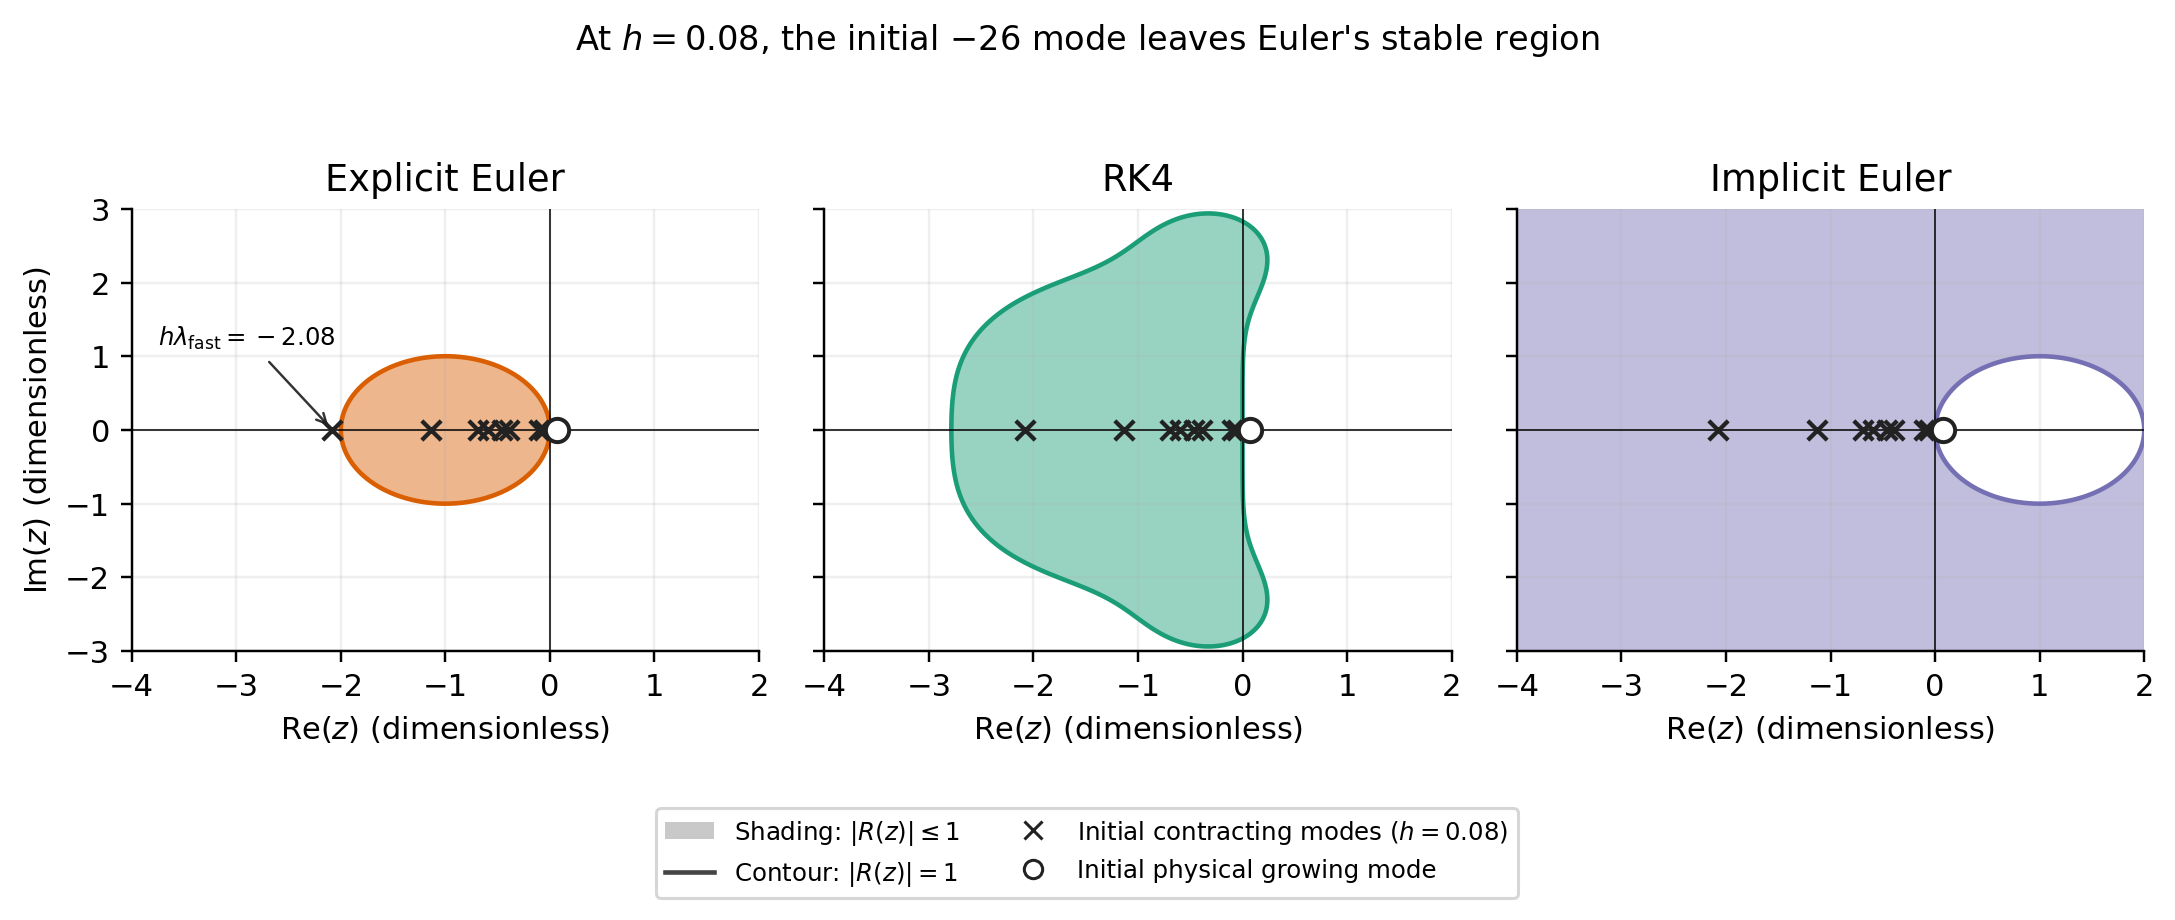
\includegraphics[width=\textwidth]{stability_regions.png}
    \caption{Absolute-stability sets $|R(z)|\leq1$ computed from the
    amplification functions. The three panels show Explicit Euler, RK4,
    and Implicit Euler, respectively. The coloured masks visualize the
    analytical regions in the dimensionless $z=h\lambda$ plane. Crosses
    locate the eight contracting eigenmodes of the initial Jacobian at
    $h=0.08$; the open circle marks the physically growing $+0.88$ mode.
    These frozen-spectrum markers do not by themselves establish
    nonlinear stability.}
    \label{fig:stability_regions}
\end{figure}

\begin{figure}[htbp]
    \centering
    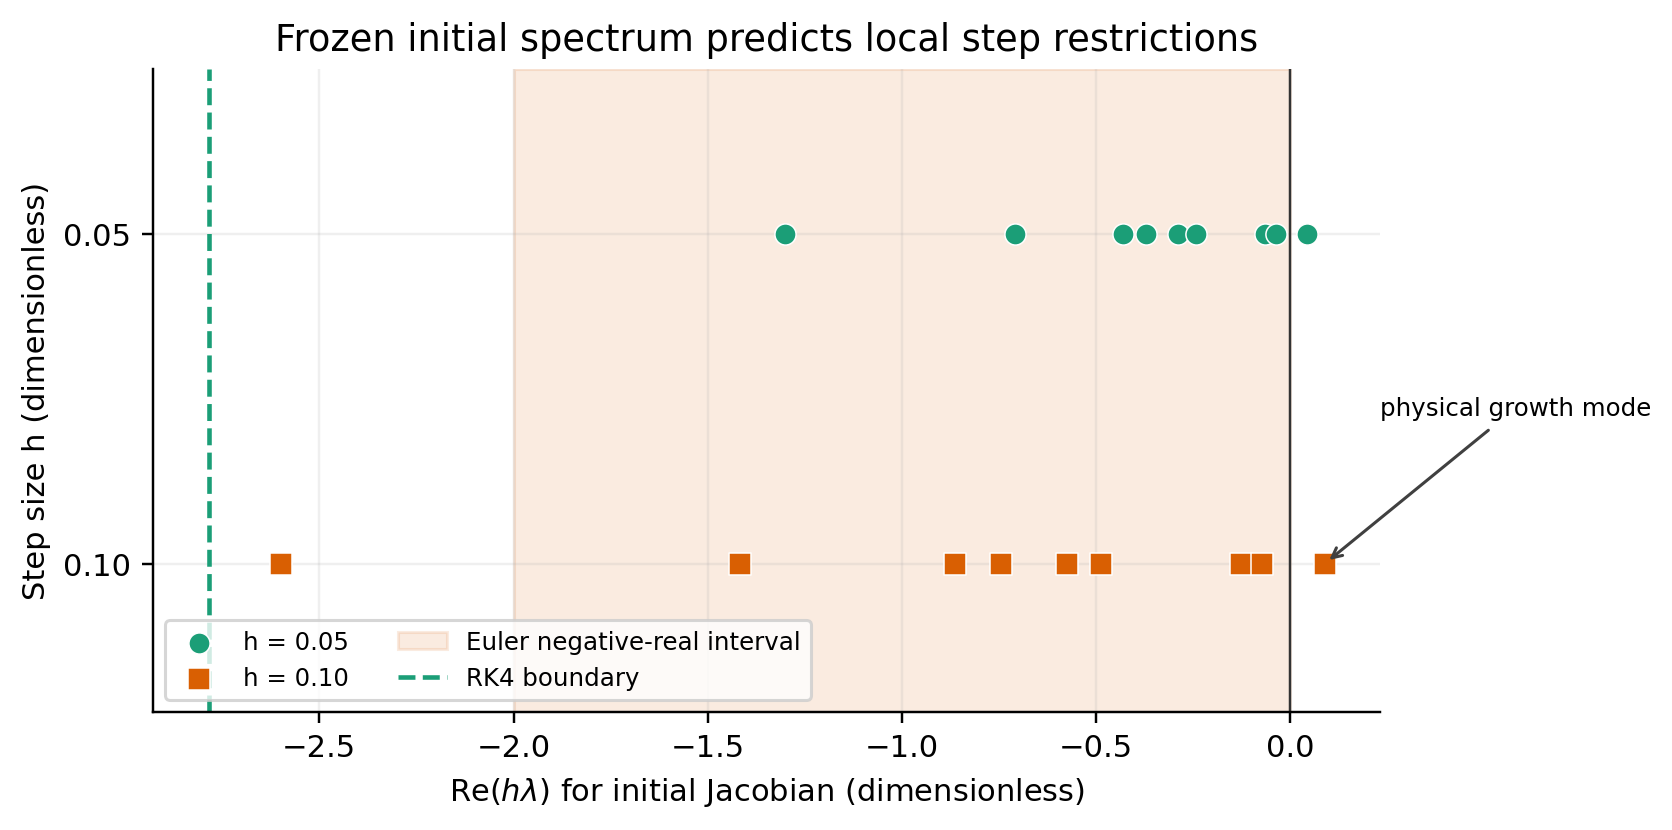
\includegraphics[width=0.78\textwidth]{frozen_spectrum.png}
    \caption{The initial Topic~5 Jacobian spectrum scaled by $h=0.05$ and
    $h=0.10$. The two categorical rows distinguish step sizes; their
    vertical positions do not represent imaginary parts. The $+0.88$
    mode reflects physical growth of the initially small singular value,
    while $h=0.10$ moves the fastest negative mode past Euler's $-2$ boundary.}
    \label{fig:frozen_spectrum}
\end{figure}

Both figures are produced by \texttt{code/experiments.py} through
\texttt{code/run\_all.py}. Figure~\ref{fig:stability_regions} shows that the
Euler disk intersects the real axis at $-2$ and $0$, while RK4 reaches
$-2.78529$ on the negative real axis and $\pm2\sqrt2$ on the imaginary
axis. The Implicit Euler panel contains the closed left half-plane, as
required by A-stability. The overlaid fastest contracting mode at
$h=0.08$ is $h\lambda_{\mathrm{fast}}=-2.08$: it falls
outside Euler's disk but inside the RK4 and Implicit Euler regions.
The open-circle mode is physical growth rather than a spurious numerical
instability. In Fig.~\ref{fig:frozen_spectrum}, the fastest
contracting Topic~5 mode gives $h\lambda_{\mathrm{fast}}=-1.30$ for $h=0.05$
and $-2.60$ for $h=0.10$. The latter lies outside the Euler interval but
inside the RK4 interval, matching the local estimates
\eqref{eq:hcrit_EE_calc}--\eqref{eq:hcrit_RK4_calc}.

\subsubsection{A-Stability and L-Stability Properties}
A numerical integration scheme is defined to be \emph{A-stable} if its region of absolute stability contains the closed left complex half-plane:
\begin{equation}
\label{eq:a_stability_def}
\mathbb{C}^- := \{ z \in \mathbb{C} : \mathrm{Re}(z) \le 0 \} \subseteq \mathcal{S}.
\end{equation}
For Implicit Euler, let $z = x + \mathrm{i}y$ with $x \le 0$. The squared modulus evaluates to:
\begin{equation}
\label{eq:a_stability_proof}
|1 - z|^2 = (1 - x)^2 + y^2 = 1 - 2x + x^2 + y^2.
\end{equation}
Since $x \le 0$, $-2x \ge 0$, and $x^2 + y^2 \ge 0$, it follows that $|1 - z|^2 \ge 1$ identically for all $z \in \mathbb{C}^-$. Therefore, Implicit Euler is unconditionally A-stable.

Furthermore, an A-stable method is classified as \emph{L-stable} if its stability function satisfies the asymptotic damping limit at stiff infinity:
\begin{equation}
\label{eq:l_stability_def}
\lim_{|z| \to \infty} |R(z)| = 0.
\end{equation}
Evaluating \eqref{eq:R_IE} gives $\lim_{|z| \to \infty} \left|\frac{1}{1 - z}\right| = 0$, confirming that Implicit Euler is L-stable. For a scalar test mode with a large negative real $h\lambda$, this strongly damps the transient. Conversely, $|R_{\mathrm{EE}}(z)|\to\infty$ and $|R_{\mathrm{RK4}}(z)|\to\infty$ as $|z|\to\infty$; their polynomial stability functions therefore cannot include the entire left half-plane. These are scalar linear-test properties and do not guarantee convergence of a nonlinear Newton solve.

\subsubsection{Problem-Specific Linearisation and Eigenvalue Spectrum (Topic 5)}
We now specialize the stability discussion to Topic~5, the polar-factor gradient flow:
\begin{equation}
\label{eq:polar_flow_spec}
\dot{\mathbf{X}} = \mathbf{f}(\mathbf{X}) = \mathbf{X}\left(\mathbf{I}_n - \mathbf{X}^T \mathbf{X}\right), \qquad \mathbf{X}(0) = \mathbf{X}_0.
\end{equation}
This is the negative gradient flow of
\begin{equation}
\label{eq:polar_lyapunov}
\Phi(\mathbf{X}) := \frac14\left\|\mathbf{X}^T\mathbf{X}-\mathbf{I}_n\right\|_F^2.
\end{equation}
Indeed, $\nabla\Phi(\mathbf{X})=\mathbf{X}(\mathbf{X}^T\mathbf{X}-\mathbf{I}_n)$ and hence
\begin{equation}
\label{eq:polar_lyapunov_decay}
\frac{\mathrm{d}}{\mathrm{d}t}\Phi(\mathbf{X}(t))
=-\left\|\mathbf{X}(t)\left(\mathbf{I}_n-\mathbf{X}(t)^T\mathbf{X}(t)\right)\right\|_F^2\le 0.
\end{equation}

For the prescribed nonsingular benchmark, let
\begin{equation}
\label{eq:topic5_benchmark}
\mathbf{X}_0=\mathbf{U}\,\mathrm{diag}(0.2,1.4,3.0)\,\mathbf{V}^T,
\qquad \mathbf{U}=R(0.4),\quad \mathbf{V}=R(-0.7),
\end{equation}
where
\begin{equation*}
R(\theta)=\begin{pmatrix}\cos\theta&-\sin\theta&0\\ \sin\theta&\cos\theta&0\\ 0&0&1\end{pmatrix}.
\end{equation*}
If
$\mathbf{X}(t)=\mathbf{U}\boldsymbol{\Sigma}(t)\mathbf{V}^T$ with
$\boldsymbol{\Sigma}(t)=\mathrm{diag}(s_1(t),\ldots,s_n(t))$, the singular vectors remain fixed and
\begin{equation}
\label{eq:singular_value_ode}
\dot{s}_i(t)=s_i(t)\left(1-s_i^2(t)\right).
\end{equation}
Solving this scalar logistic equation gives the exact finite-time singular values
\begin{equation}
\label{eq:singular_value_exact}
s_i(t)=\frac{s_{i,0}}{\sqrt{s_{i,0}^2+\left(1-s_{i,0}^2\right)e^{-2t}}}.
\end{equation}
Thus $0<s_{i,0}<1$ gives monotone increase to $1$, $s_{i,0}>1$ gives monotone decrease to $1$, and $s_{i,0}=0$ remains zero. Scalar solutions cannot cross, so the ordering of the singular values is preserved. For a rank-deficient initial matrix, the limiting matrix is therefore a partial isometry rather than an orthogonal matrix. These facts provide exact diagnostics for the numerical experiments. As an independent sanity check, a positive diagonal initial matrix remains diagonal and each entry follows \eqref{eq:singular_value_exact}; this case is checked against the numerical RK4 trajectory in \texttt{test/test\_validation.py}.

The Fr\'echet derivative in a matrix direction $\mathbf{H}$ is the
operator already derived in \eqref{eq:topic5_frechet_derivative}.
Using column-major vectorisation, $\mathrm{vec}(\mathbf{A}\mathbf{B}\mathbf{C})=(\mathbf{C}^T\otimes\mathbf{A})\mathrm{vec}(\mathbf{B})$ and $\mathrm{vec}(\mathbf{H}^T)=\mathbf{K}_{n,n}\mathrm{vec}(\mathbf{H})$, this becomes
\begin{equation}
\label{eq:analytic_jacobian_kron}
\mathbf{J}_{\mathbf{f}}(\mathbf{X})
=\mathbf{I}_n\otimes\left(\mathbf{I}_n-\mathbf{X}\mathbf{X}^T\right)
-\left(\mathbf{X}^T\otimes\mathbf{X}\right)\mathbf{K}_{n,n}
-\left(\mathbf{X}^T\mathbf{X}\right)^T\otimes\mathbf{I}_n.
\end{equation}
If a row-major vectorisation is used in code, the corresponding permutation of this Jacobian must be used instead.

For the spectral calculation write $\mathbf{X}=\mathbf{U}\boldsymbol{\Sigma}\mathbf{V}^T$ and $\mathbf{H}=\mathbf{U}\mathbf{K}\mathbf{V}^T$. Then the transformed linearised operator is
\begin{equation}
\label{eq:svd_linearised_operator}
\mathcal{L}_{\boldsymbol{\Sigma}}[\mathbf{K}]
=\mathbf{K}(\mathbf{I}_n-\boldsymbol{\Sigma}^2)
-\boldsymbol{\Sigma}(\mathbf{K}^T\boldsymbol{\Sigma}+\boldsymbol{\Sigma}\mathbf{K}).
\end{equation}
The diagonal directions have eigenvalues
\begin{equation}
\label{eq:diagonal_jacobian_eigenvalues}
\lambda_{ii}=1-3s_i^2.
\end{equation}
For each pair $i<j$, the $(K_{ij},K_{ji})$ block is
\begin{equation}
\label{eq:offdiagonal_jacobian_eigenvalues}
\begin{pmatrix}
1-s_i^2-s_j^2 & -s_i s_j \\
-s_i s_j & 1-s_i^2-s_j^2
\end{pmatrix}.
\end{equation}
The eigenvector $(1,1)^T$ represents a symmetric perturbation,
whereas $(1,-1)^T$ represents a skew-symmetric perturbation. Thus
\begin{align}
\lambda_{ij}^{\mathrm{sym}}
&=1-s_i^2-s_j^2-s_i s_j, \\
\lambda_{ij}^{\mathrm{skew}}
&=1-s_i^2-s_j^2+s_i s_j.
\end{align}
At an orthogonal equilibrium $s_i=1$, these formulas give
$\lambda_{ij}^{\mathrm{sym}}=-2$ and
$\lambda_{ij}^{\mathrm{skew}}=0$. Hence symmetric perturbations are
contracting normal directions, whereas skew-symmetric perturbations are
neutral tangent directions along the manifold of orthogonal equilibria.
The neutral tangent space has dimension $n(n-1)/2$ and the contracting
normal space has dimension $n(n+1)/2$.

For the benchmark in \eqref{eq:topic5_benchmark}, the full frozen Jacobian spectrum is
\begin{equation}
\label{eq:topic5_initial_spectrum}
\sigma\left(\mathbf{J}_{\mathbf{f}}(\mathbf{X}_0)\right)
=\{0.88,-0.72,-1.28,-4.88,-5.76,-7.44,-8.64,-14.16,-26.0\}.
\end{equation}
The positive eigenvalue $0.88$ represents the physical growth of the singular value $s_1=0.2$ toward $1$; it is not a numerical instability. The fastest contracting mode is $-26$, generated by $s_3=3$, while the slowest negative mode is $-0.72$. Thus a decay-rate spread based on the negative modes is $26/0.72\approx36.1$, and the transient should be described as a multiscale problem rather than as a spectrum that is entirely negative.

\subsubsection{Theoretical Step-Size Limits vs. Empirical Disclaimers}
At the initial state, mapping the fastest contracting spectral point $\lambda_{\mathrm{fast}}=-26.0$ onto the real stability intervals gives local frozen-Jacobian step-size estimates for the explicit solvers:
\begin{align}
\text{Explicit Euler:} \quad & h_{\mathrm{crit}}^{\mathrm{EE}} = \frac{2}{|\lambda_{\mathrm{fast}}|} = \frac{2}{26.0} \approx 0.0769, \label{eq:hcrit_EE_calc} \\
\text{Classical RK4:} \quad & h_{\mathrm{crit}}^{\mathrm{RK4}} = \frac{2.78529}{|\lambda_{\mathrm{fast}}|} = \frac{2.78529}{26.0} \approx 0.1071. \label{eq:hcrit_RK4_calc}
\end{align}
Figure~\ref{fig:frozen_spectrum} overlays the absolute-stability cutoffs
with the scaled frozen-Jacobian eigenvalues $z_j=h\lambda_j$ at two
representative step sizes. It is a local diagnostic at $\mathbf{X}_0$:
because the spectrum changes along the nonlinear trajectory, it cannot
replace the step-size sweeps and perturbation experiments required for a
global numerical claim.

\paragraph{Mandatory Analytical Disclaimer:}
\emph{We formally emphasize that the $h\lambda$ spectral overlay represents a local frozen-Jacobian diagnostic rather than a global nonlinear stability proof. Because the Jacobian $\mathbf{J}_{\mathbf{f}}(\mathbf{X}(t))$ varies continuously along the matrix trajectory, frozen-eigenvalue containment $|R(h\lambda_j)| \le 1$ is only a local condition and does not prove global nonlinear convergence. Finite-step nonlinear effects can still violate monotonicity or positivity properties. Consequently, the estimates \eqref{eq:hcrit_EE_calc}--\eqref{eq:hcrit_RK4_calc} must be tested by systematic step-size sweeps and perturbation experiments.}

\subsection{Convergence}

\label{sec:convergence}

Having established the consistency orders in Section~\ref{sec:consistency_and_truncation_error} and linear stability boundaries in Section~\ref{sec:stability_analysis}, we now unify these components to prove the global convergence of the numerical trajectory towards the theoretical solution.

\subsubsection{Discrete Error Recurrence and the Discrete Gr\"onwall Lemma}
Let $\mathbf{y}(t) \in C^{p+1}[t_0, T]$ be the exact continuous trajectory of the initial value problem \eqref{eq:general_ivp}, and let $\{\mathbf{y}_n\}_{n=0}^N$ be the discrete numerical approximation generated by the one-step scheme:
\begin{equation}
\label{eq:increment_form_convergence}
\mathbf{y}_{n+1} = \mathbf{y}_n + h \mathbf{\Phi}(t_n, \mathbf{y}_n, h), \quad \mathbf{y}_0 = \mathbf{y}(t_0),
\end{equation}
where $h = (T - t_0)/N$. The true solution identically satisfies the perturbed relation:
\begin{equation}
\label{eq:exact_perturbed_relation}
\mathbf{y}(t_{n+1}) = \mathbf{y}(t_n) + h \mathbf{\Phi}(t_n, \mathbf{y}(t_n), h) + h \boldsymbol{\tau}_{n+1},
\end{equation}
where $\boldsymbol{\tau}_{n+1}$ is the local truncation error vector defined in \eqref{eq:lte_def}. We assume that the increment function $\mathbf{\Phi}$ is uniformly Lipschitz in its state argument on a bounded neighborhood $\Omega$ containing the exact and numerical trajectories, with an effective Lipschitz constant $\Lambda>0$ independent of sufficiently small $h$. Consequently, the one-step map $G_h(t,\mathbf{u})=\mathbf{u}+h\mathbf{\Phi}(t,\mathbf{u},h)$ has Lipschitz factor at most $1+h\Lambda$. For Implicit Euler, this additionally requires existence of the selected nonlinear root and a uniformly bounded inverse of the residual Jacobian. More precisely, assume that for some $M_J$ independent of sufficiently small $h$,
\begin{equation}
\label{eq:uniform_residual_inverse}
\sup_{\substack{(t,\mathbf{w})\in\Omega\\ t+h\le T}}
\left\|
\left(\mathbf{I}_d-h\mathbf{J}_{\mathbf f}(t+h,\mathbf{w})\right)^{-1}
\right\|\le M_J.
\end{equation}
This condition controls the sensitivity of the selected nonlinear root to perturbations in the accepted state. We then impose the increment Lipschitz bound:
\begin{equation}
\label{eq:increment_lipschitz}
\|\mathbf{\Phi}(t, \mathbf{u}, h) - \mathbf{\Phi}(t, \mathbf{v}, h)\| \le \Lambda \|\mathbf{u} - \mathbf{v}\|, \quad \forall (t, \mathbf{u}), (t, \mathbf{v}) \in \Omega, \; \forall h \in (0, h_0].
\end{equation}
We define the global discretization error at grid node $t_n$ as:
\begin{equation}
\label{eq:global_error_def}
\mathbf{e}_n := \mathbf{y}(t_n) - \mathbf{y}_n, \quad n = 0, 1, \dots, N.
\end{equation}
Subtracting \eqref{eq:increment_form_convergence} from \eqref{eq:exact_perturbed_relation} yields the dynamic recurrence for the error vector:
\begin{equation}
\label{eq:error_recurrence_vector}
\mathbf{e}_{n+1} = \mathbf{e}_n + h \left[ \mathbf{\Phi}(t_n, \mathbf{y}(t_n), h) - \mathbf{\Phi}(t_n, \mathbf{y}_n, h) \right] + h \boldsymbol{\tau}_{n+1}.
\end{equation}
Taking Euclidean norms on both sides of \eqref{eq:error_recurrence_vector} and applying the triangle inequality alongside \eqref{eq:increment_lipschitz}:
\begin{align}
\|\mathbf{e}_{n+1}\| &\le \|\mathbf{e}_n\| + h \|\mathbf{\Phi}(t_n, \mathbf{y}(t_n), h) - \mathbf{\Phi}(t_n, \mathbf{y}_n, h)\| + h \|\boldsymbol{\tau}_{n+1}\| \nonumber \\
&\le \|\mathbf{e}_n\| + h \Lambda \|\mathbf{y}(t_n) - \mathbf{y}_n\| + h \|\boldsymbol{\tau}_{n+1}\| \nonumber \\
&= (1 + h \Lambda) \|\mathbf{e}_n\| + h \|\boldsymbol{\tau}_{n+1}\|. \label{eq:scalar_error_inequality}
\end{align}
Let $\tau_{\max}(h) := \max_{1 \le k \le N} \|\boldsymbol{\tau}_k\|$. Unrolling the scalar recurrence \eqref{eq:scalar_error_inequality} inductively from the initial state yields:
\begin{equation}
\label{eq:unrolled_error_sum}
\|\mathbf{e}_n\| \le (1 + h\Lambda)^n \|\mathbf{e}_0\| + h \tau_{\max}(h) \sum_{j=0}^{n-1} (1 + h\Lambda)^j.
\end{equation}
Assuming exact initial data ($\|\mathbf{e}_0\| = 0$) and summing the finite geometric progression with ratio $1 + h\Lambda > 1$:
\begin{equation}
\label{eq:geometric_sum_evaluation}
\sum_{j=0}^{n-1} (1 + h\Lambda)^j = \frac{(1 + h\Lambda)^n - 1}{(1 + h\Lambda) - 1} = \frac{(1 + h\Lambda)^n - 1}{h\Lambda}.
\end{equation}
Substituting \eqref{eq:geometric_sum_evaluation} into \eqref{eq:unrolled_error_sum}, and noting the fundamental inequality $1 + x \le e^x$ for all $x \ge 0$, we have:
\begin{equation}
\label{eq:exponential_upper_bound}
(1 + h\Lambda)^n \le \left(e^{h\Lambda}\right)^n = e^{n h \Lambda} = e^{\Lambda (t_n - t_0)} \le e^{\Lambda(T - t_0)}.
\end{equation}
Combining \eqref{eq:unrolled_error_sum}--\eqref{eq:exponential_upper_bound} produces the classical discrete Gr\"onwall bound on the global discretization error (with the continuous limit understood when $\Lambda=0$):
\begin{equation}
\label{eq:global_convergence_bound}
\|\mathbf{e}_n\| \le \frac{e^{\Lambda(T - t_0)} - 1}{\Lambda} \tau_{\max}(h), \quad \forall n = 0, 1, \dots, N.
\end{equation}

\subsubsection{Global Convergence Order}
The bound \eqref{eq:global_convergence_bound} provides the fundamental mathematical bridge between the local truncation error rate $\boldsymbol{\tau}$ and the global error $\mathbf{e}_n$:
\begin{itemize}
    \item \textbf{Explicit / Implicit Euler ($p=1$):} Since $\|\boldsymbol{\tau}_{n+1}\| \le C_1 h$, the terminal error satisfies:
    \begin{equation}
    \label{eq:euler_global_order}
    \|\mathbf{e}_N\| \le \left( \frac{e^{\Lambda(T - t_0)} - 1}{\Lambda} C_1 \right) h = \mathcal{O}(h).
    \end{equation}
    \item \textbf{Classical Runge--Kutta (RK4, $p=4$):} Since $\|\boldsymbol{\tau}_{n+1}\| \le C_4 h^4$, the terminal error satisfies:
    \begin{equation}
    \label{eq:rk4_global_order}
    \|\mathbf{e}_N\| \le \left( \frac{e^{\Lambda(T - t_0)} - 1}{\Lambda} C_4 \right) h^4 = \mathcal{O}(h^4).
    \end{equation}
\end{itemize}
The preceding estimates assume that the nonlinear equation in each
Implicit Euler step is solved sufficiently accurately. If the Newton
iteration is stopped with an algebraic residual larger than the
time-discretisation error, the observed rate can be limited by the
nonlinear-solver tolerance rather than by the formal order of the
time-stepping method. In computations, the Newton residual tolerance
must therefore be chosen below the target time-discretisation error.

This explains the apparent paradox regarding order indices: while an individual integration step generates a local defect of order $\mathcal{O}(h^{p+1})$, the accumulation of $N = \mathcal{O}(h^{-1})$ steps over a compact temporal interval $[t_0, T]$ causes the discrete sequence to converge globally at order $\mathcal{O}(h^p)$.

For standard one-step methods, consistency together with a uniform Lipschitz stability bound implies convergence. In the present setting this is exactly the role of the estimate above; the multistep characteristic-polynomial root condition is not needed for Explicit Euler, RK4, or Implicit Euler.

\subsubsection{Implications for Empirical Log-Log Validation}
For Topic~5, the finite-time exact matrix solution associated with the
benchmark in \eqref{eq:topic5_benchmark} is
\begin{equation}
\label{eq:topic5_exact_matrix_solution}
\mathbf{X}_{\mathrm{exact}}(t)
=
\mathbf{U}\,\operatorname{diag}\bigl(s_1(t),\ldots,s_n(t)\bigr)\,\mathbf{V}^T,
\end{equation}
where the singular values are given by \eqref{eq:singular_value_exact}.
The terminal numerical error is measured in the Frobenius norm:
\begin{equation}
\label{eq:topic5_frobenius_error}
E_h(T)=\left\|\mathbf{X}_h(T)-\mathbf{X}_{\mathrm{exact}}(T)\right\|_F.
\end{equation}
Let $\mathcal{E}_h=\|\mathbf{e}_N(h)\|$ for the vector formulation
and $\mathcal{E}_h=E_h(T)$ for Topic~5. Taking the natural logarithm of
the asymptotic relation $\mathcal{E}_h\approx C h^p$ yields:
\begin{equation}
\label{eq:loglog_linear_relation}
\ln \mathcal{E}_h \approx p \ln h + \ln C.
\end{equation}
Equation \eqref{eq:loglog_linear_relation} establishes that plotting the
terminal error (using $E_h(T)$ for Topic~5) against the discretisation
step size on a logarithmic scale yields an affine straight line whose
asymptotic slope is the theoretical convergence order $p$. In the
numerical-experiments section, this relation serves as the primary
quantitative metric for Explicit Euler ($p\approx1$), Implicit Euler
($p\approx1$), and classical RK4 ($p\approx4$).
For two consecutive step sizes $h$ and $h/2$, the observed order is
estimated by
\begin{equation}
\label{eq:observed_order}
p_{\mathrm{obs}}(h)
=
\frac{\log\left(E_h(T)/E_{h/2}(T)\right)}{\log 2}.
\end{equation}
Thus the expected asymptotic values are $p_{\mathrm{obs}}\approx1$ for
Explicit and Implicit Euler and $p_{\mathrm{obs}}\approx4$ for RK4.

\newpage
% ============================================================

\section{Implementation}
% ============================================================

\subsection{Algorithm}
The three one-step updates are \eqref{eq:explicit_euler},
\eqref{eq:rk4_update}, and \eqref{eq:implicit_euler}; the last calls
Algorithm~\ref{alg:implicit_euler_newton}. For a fixed-grid convergence
run, the implementation chooses an integer $N$, sets
$h=(T-t_0)/N$, and performs exactly $N$ updates. A failed nonlinear
solve raises an error so that no grid is silently changed.
Algorithm~\ref{alg:adaptive} describes the separate adaptive
controller implemented for all three base methods. A standard
treatment of these one-step methods appears in \cite{hairer1993}.

\begin{algorithm}[htbp]
\caption{Step-doubling adaptive integration}
\label{alg:adaptive}
\footnotesize
\begin{algorithmic}[1]
\Require Method $\Psi_h$ of order $p$; $t_0,\mathbf y_0,T,h$;
  $\mathrm{atol}>0$, $\mathrm{rtol}\geq0$.
\Ensure Accepted trajectory ending at $T$, or a reported failure.
\State $(t,\mathbf y)\gets(t_0,\mathbf y_0)$
\While{$t<T$ and the trial limit is not exhausted}
    \State $h\gets\min\{h,T-t\}$
    \If{$h$ falls below the permitted minimum away from the final endpoint}
        \State \Return failure
    \EndIf
    \State Try $\mathbf y_c=\Psi_h(t,\mathbf y)$,
      $\mathbf y_m=\Psi_{h/2}(t,\mathbf y)$, and
      $\mathbf y_f=\Psi_{h/2}(t+h/2,\mathbf y_m)$
    \If{a nonlinear one-step solve reports failure}
        \State Reject; $h\gets h/2$; \textbf{continue} from $(t,\mathbf y)$
    \EndIf
    \State $\widehat{\mathbf e}\gets
      (\mathbf y_f-\mathbf y_c)/(2^p-1)$
    \State $s_i\gets \mathrm{atol}+
      \mathrm{rtol}\max\{|y_i|,|y_{f,i}|\}$;
      $E\gets\max_i|\widehat e_i|/s_i$
    \If{$E$ is non-finite}
        \State $E\gets\infty$
    \EndIf
    \If{$E\leq1$}
        \State Accept: $(t,\mathbf y)\gets(t+h,\mathbf y_f)$;
          store the time, state, actual $h$, and $E$
        \If{$t=T$}
            \State \Return accepted trajectory
        \EndIf
    \Else
        \State Reject; keep $(t,\mathbf y)$ unchanged
    \EndIf
    \State $r\gets 2$ if $E=0$; otherwise
      $r\gets\operatorname{clip}(0.9E^{-1/(p+1)},0.2,2)$
    \State $h\gets rh$
\EndWhile
\State \Return failure if $T$ was not reached
\end{algorithmic}
\end{algorithm}

\subsection{Code Structure}
\begin{table}[H]
\centering
\begin{tabular}{lp{0.68\textwidth}}
\toprule
\textbf{File} & \textbf{Purpose} \\
\midrule
\texttt{code/model.py} & Topic~5 benchmark, column-major vectorization,
  matrix RHS, analytic Jacobian, exact SVD solution, and diagnostics. \\
\texttt{code/solvers.py} & Explicit Euler, RK4, Implicit Euler with
  damped Newton, fixed-grid and adaptive drivers, and work counters. \\
\texttt{code/experiments.py} & Convergence, reference, stability,
  trajectory, adaptivity, cost, and rank-deficient experiments;
  exports PNGs to \path{figures/}, and CSV/JSON to \path{data/}. \\
\texttt{code/run\_all.py} & One command regenerates every report figure. \\
\texttt{code\_zh/} & Independently runnable Chinese-commented version of
  the same four modules. \\
\texttt{test/} & Model, order, geometry, adaptivity, and bilingual
  parity checks for all three methods. \\
\texttt{report\_v2/data/} & Frozen CSV/JSON evidence documented in Appendix~\ref{sec:appendix_c}. \\
\bottomrule
\end{tabular}
\caption{Files used to reproduce the numerical results.}
\label{tab:code_structure}
\end{table}


\subsection{Output Layout and Reproduction}
Run \texttt{python code/run\_all.py} from \path{Project1/}.
The source directory contains only source and documentation.
Eight regenerated images are written to the sibling \path{figures/}
directory, while six CSV files and \path{summary.json} are written
to \path{data/}. The Chinese-commented implementation is independently
run with \texttt{python code\_zh/run\_all.py}; its isolated outputs are in
\path{outputs_zh/figures/} and \path{outputs_zh/data/}.
All paths are resolved from the entry-point file rather than a
machine-specific drive or the shell's current directory.

This report version bundles its own \path{figures/} and \path{data/}
snapshots. Appendix~\ref{sec:appendix_c} maps every evidence file to
its figures, fields, and claims. Reproduction writes to the project-level
output directories; it does not overwrite archived report versions.
\texttt{python -B -m unittest discover -s test -v} runs the numerical
and bilingual checks. The version index in
\path{notes/REPORT_VERSIONS.md} identifies the current report and
the Git tags used to recover earlier complete project states.

\subsection{Key Design Decisions}
The state is a nine-component column-major vector
$\operatorname{vec}(X)$ throughout. The analytic Fr\'echet derivative
\eqref{eq:topic5_frechet_derivative} supplies Newton's Jacobian;
Newton starts from the previous accepted state and uses the
scale-aware residual threshold
$\|F(w)\|_\infty\leq10^{-12}(1+\|w\|_\infty)$.
Backtracking accepts only a finite candidate whose \emph{complete}
residual decreases. The adaptive controller accepts two half steps,
not a Richardson-corrected state, so its base method retains order
$p$. It reports accepted and rejected trials separately. The exact
SVD solution is excluded from all solver steps and is used only for
validation; an independently integrated Radau trajectory through
SciPy provides a second check \cite{virtanen2020}. Both English- and Chinese-commented implementations
generate the same numerical summary. Dependencies, invocation
commands, and every generated figure are documented in the two
README files.

As an independent check of the implicit-step Jacobian, we use the
benchmark vector $y_0=\operatorname{vec}(X_0)$, $h=0.05$, and direction
$v=(0.1,0.2,\ldots,0.9)^T$. With
$F(w)=w-y_0-hf(h,w)$ and $\varepsilon=10^{-6}$, the centred difference
$[F(y_0+\varepsilon v)-F(y_0-\varepsilon v)]/(2\varepsilon)$ differs
from $(I-hJ_f(y_0))v$ by $3.68\times10^{-10}$ in the infinity norm.
This checks the complete residual derivative, including the identity
term; the reproducible calculation is in
\texttt{test/test\_validation.py}.

\newpage
% ============================================================

\section{Numerical Experiments}
% ============================================================

\subsection{Verification Against the Exact Matrix}
We integrate the prescribed $X_0$ over $[0,2]$ on fixed uniform grids
and measure the full-matrix terminal error
\[
E_h(2)=\|X_h(2)-X_{\rm exact}(2)\|_F.
\]
The limiting orthogonal factor is not the finite-time reference.
Euler and Implicit Euler use $N\in\{40,80,160,320\}$.
RK4 also uses $N\in\{640,1280,2560\}$.
The finest three RK4 grids are used for the displayed slope because
the coarse-grid ratios are affected by the rapid initial transient.
The smallest measured error is near floating-point round-off scale,
so the fitted fine-grid slope is a descriptive validation diagnostic;
no flat round-off floor has been observed on these grids. Table~\ref{tab:order_results} and
Fig.~\ref{fig:convergence} report the measured orders.

\begin{table}[htbp]
\centering
\begin{tabular}{lrrr}
\toprule
Method & Fitted slope & Finest $h$ & Finest terminal error \\
\midrule
Explicit Euler & $1.010$ & $0.00625$ & $4.6141\times10^{-4}$ \\
RK4 & $3.927$ & $0.00078125$ & $7.3968\times10^{-14}$ \\
Implicit Euler & $1.014$ & $0.00625$ & $4.6429\times10^{-4}$ \\
\bottomrule
\end{tabular}
\caption{Finite-time full-matrix Frobenius error. The complete
grid-by-grid values and adjacent observed orders are in
\texttt{data/convergence.csv}.}
\label{tab:order_results}
\end{table}

\begin{figure}[htbp]
\centering
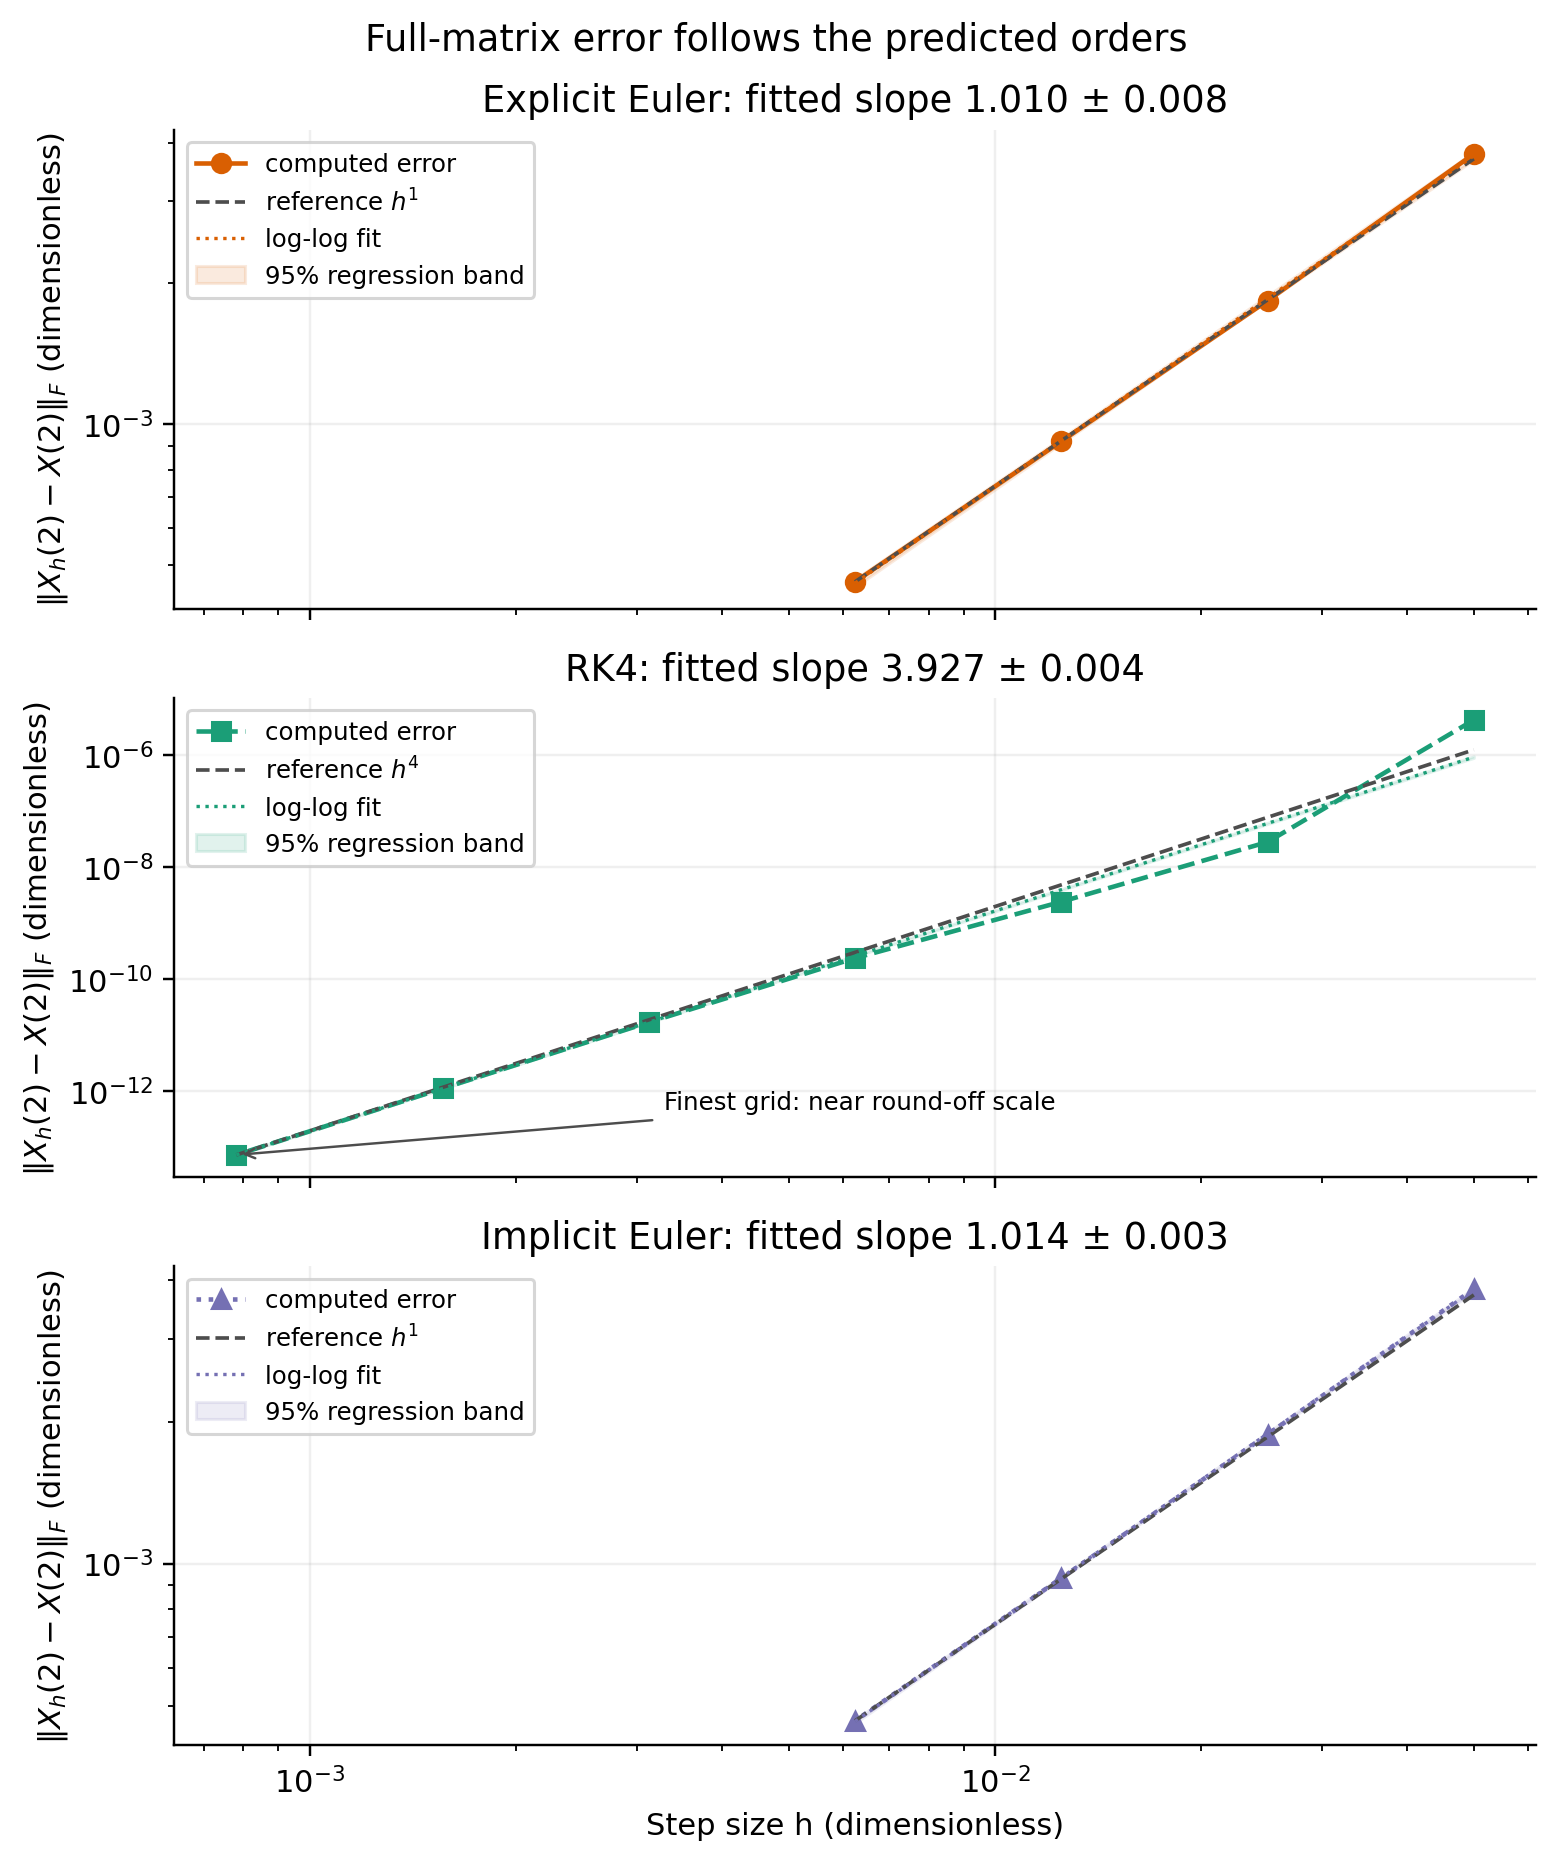
\includegraphics[width=0.76\textwidth]{convergence.png}
\caption{Terminal full-matrix error versus dimensionless step size, with
$h^1$ or $h^4$ reference slopes and fitted slopes from the refined grids.
The shaded 95\% regression bands and reported slope standard errors are
descriptive least-squares diagnostics for deterministic mesh data, not
probabilistic uncertainty in the ODE solution. The agreement verifies the
predicted global orders against the finite-time exact matrix.}
\label{fig:convergence}
\end{figure}

A separate \texttt{solve\_ivp} Radau run with relative tolerance
$10^{-12}$ and absolute tolerance $10^{-14}$ differs from the exact
SVD matrix at $t=2$ by $1.16\times10^{-13}$ in Frobenius norm. This
cross-check and the analytic formula are independent of the three
implemented time-stepping methods.

\subsection{Stability Experiments}
The initial frozen-Jacobian estimates
$h_{\rm crit}^{\rm EE}\approx0.0769$ and
$h_{\rm crit}^{\rm RK4}\approx0.1071$ predict the onset of possible
amplification in the fastest contracting direction. We test selected
fixed steps $h=2/N$ with $N=6,7,8,10,12,16,20,24,32,40,50,64,80$
and perturb the initial state by $10^{-7}$ in that direction.
At $h=0.10$, one Euler step amplifies this perturbation by about $1.60$,
although the full numerical path still finishes. At $h=2/7$, Euler
increases $\Phi$ by $31.9$ on its first step and the run subsequently
fails. RK4 at $h=1/3$ also fails after a large first-step energy rise,
whereas Implicit Euler finishes that tested grid. These observations
support the predicted local risk but do not turn the frozen-eigenvalue
cutoffs into nonlinear global thresholds.

\begin{figure}[htbp]
\centering
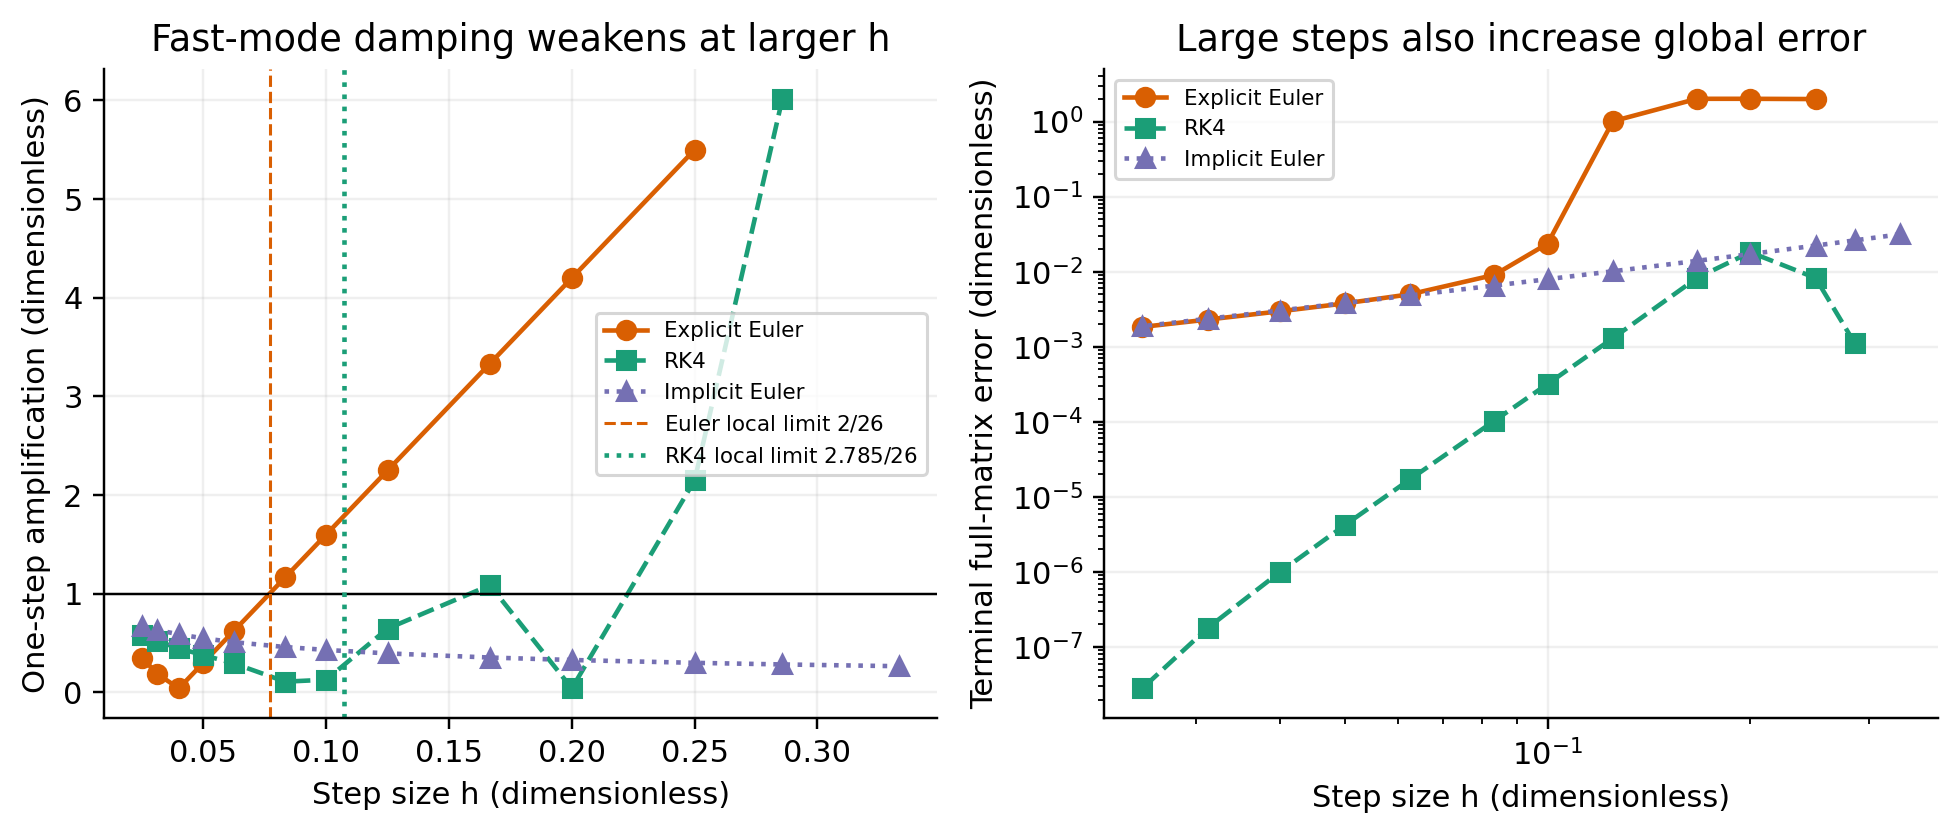
\includegraphics[width=0.85\textwidth]{stability_sweep.png}
\caption{Left: one-step amplification of a fast-direction initial
perturbation. Right: terminal error for completed runs on log--log axes. The labelled
vertical lines show Euler and RK4 limits from the initial frozen
Jacobian; they are local estimates, so the nonlinear sweep is needed
to assess their relevance. Energy changes and failed-run statuses are in
\texttt{stability\_sweep.csv}.}
\label{fig:stability_sweep}
\end{figure}

\subsection{Adaptivity}
For all three base methods, the step-doubling trials start at $h=0.15$
with $\mathrm{atol}=10^{-8}$ and $\mathrm{rtol}=10^{-6}$.
The fine result is accepted only when its normalized estimated local
error is at most one. Table~\ref{tab:adaptive_results} and
Fig.~\ref{fig:adaptive_steps} show that the accepted step size genuinely
changes. A very short final step may be caused by clipping to reach
$t=2$ exactly. These local tolerances do not provide a strict bound on
the terminal global error, which we measure separately against the
exact SVD matrix.

\begin{table}[htbp]
\centering
\begin{tabular}{lrrrr}
\toprule
Method & Accepted & Rejected & Max.\ accepted $E$ & Terminal error \\
\midrule
Explicit Euler & 1680 & 5 & $0.842$ & $5.08\times10^{-5}$ \\
RK4 & 17 & 2 & $0.754$ & $6.89\times10^{-7}$ \\
Implicit Euler & 1678 & 5 & $0.843$ & $5.09\times10^{-5}$ \\
\bottomrule
\end{tabular}
\caption{Step-doubling runs with the same local tolerance settings.
The numbers of accepted steps alone are not a work comparison:
each trial computes one full and two half steps, and rejected trials
also consume evaluations.}
\label{tab:adaptive_results}
\end{table}

\begin{figure}[htbp]
\centering
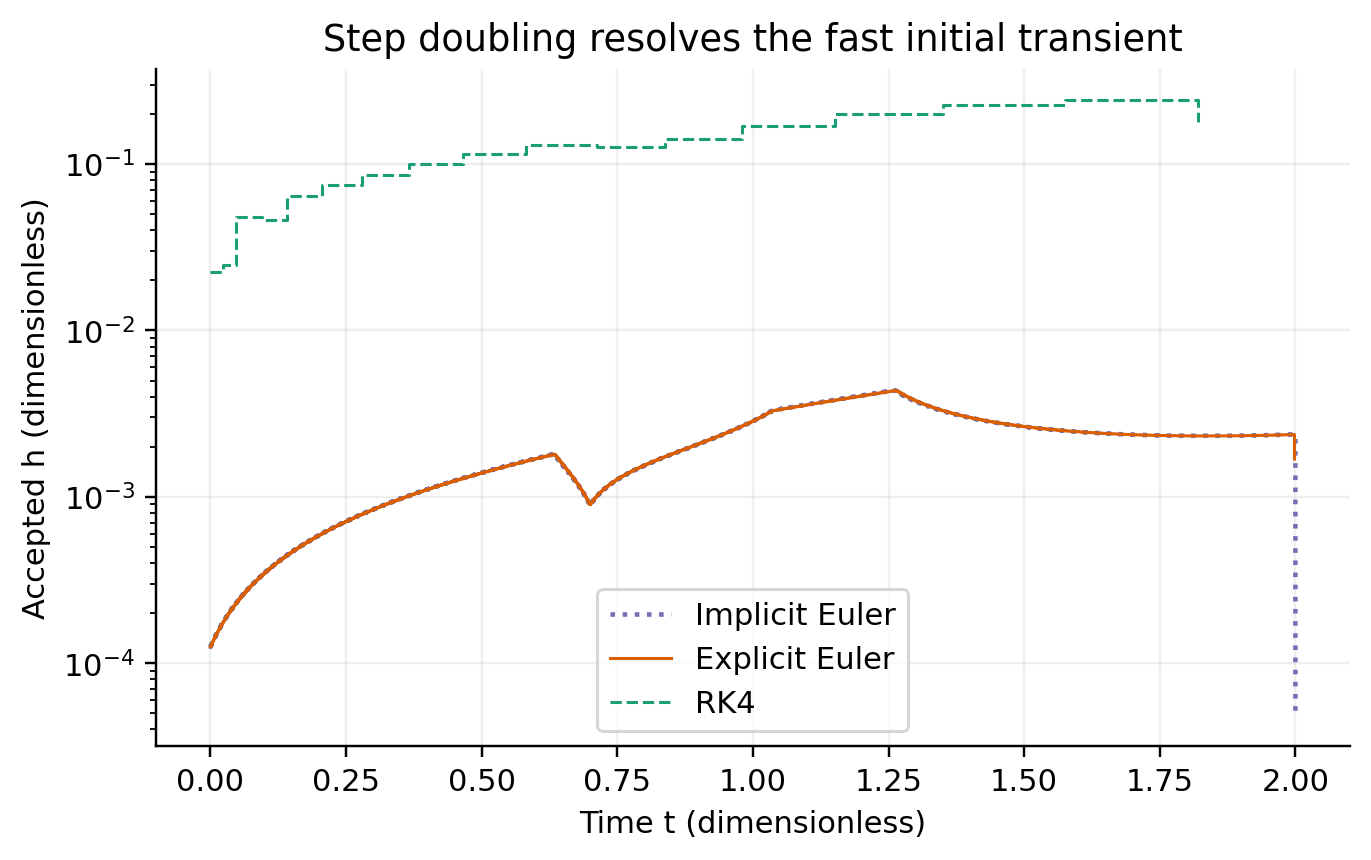
\includegraphics[width=0.78\textwidth]{adaptive_steps.png}
\caption{Accepted step length versus dimensionless time. Step doubling
reduces the step during the rapid initial transient; the accepted-step
data and estimated local error are in \texttt{adaptive\_steps.csv}.}
\label{fig:adaptive_steps}
\end{figure}

\subsection{Main Results and Comparison of Methods}
\paragraph{Geometry and Lyapunov diagnostics.}
On the RK4 trajectory with $h=0.005$, every sampled singular value
moves toward one without crossing it, and $\Phi(X)$ decreases at every
stored step. The numerical orthogonality defect at $t=2$ is
$0.305932824226$, compared with the nonzero exact finite-time value
$0.305932824210$. Figure~\ref{fig:trajectory_diagnostics} also shows
the finite-difference check of
$\mathrm d\Phi/\mathrm dt=-\|X(I-X^TX)\|_F^2$.
Its maximum absolute residual is about $0.240$, concentrated in the
initial fast transient; the maximum residual scaled by
$\max(1,|\mathrm d\Phi/\mathrm dt|)$ is $4.69\times10^{-4}$.
This is a discrete diagnostic, not a direct test that the continuous
identity fails.

\begin{figure}[htbp]
\centering
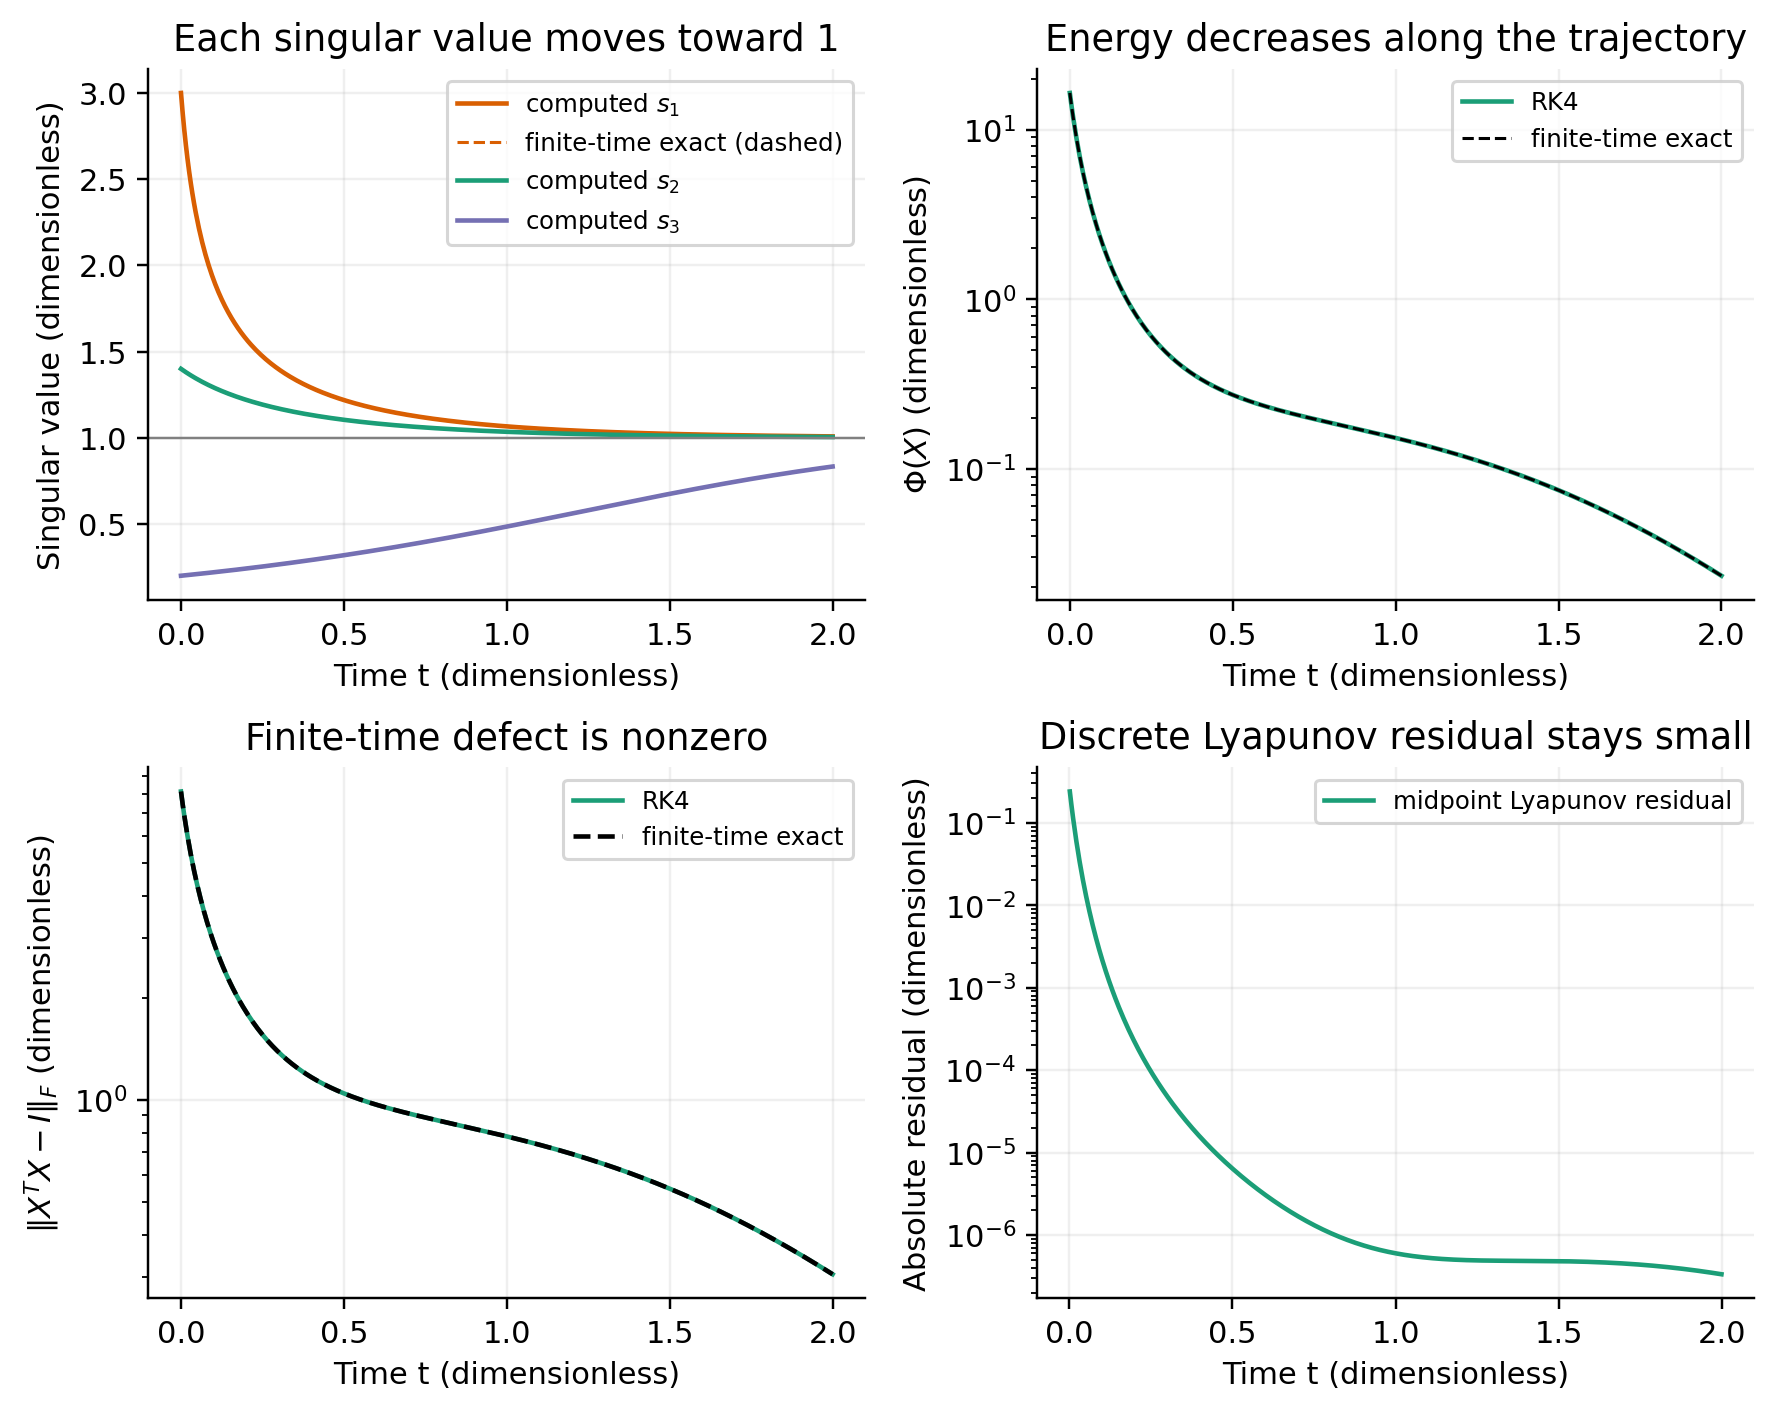
\includegraphics[width=\textwidth]{trajectory_diagnostics.png}
\caption{Singular values, Lyapunov energy, finite-time orthogonality
defect, and the discrete identity residual along a resolved RK4
trajectory. Dashed curves give the finite-time exact SVD reference for
the first three panels; the fourth panel explicitly labels the
midpoint Lyapunov residual. Their overlap confirms accuracy while the
nonzero exact defect explains why finite-time orthogonality is not expected.}
\label{fig:trajectory_diagnostics}
\end{figure}

\paragraph{Cost at comparable accuracy.}
We select fixed grids that yield terminal full-matrix errors within
$5.4\%$ of one another, then count RHS evaluations as the common
work measure. Table~\ref{tab:cost_accuracy} and
Fig.~\ref{fig:cost_accuracy} show that RK4 needs fewer RHS calls for
this target, while Implicit Euler incurs many nonlinear-solver calls.
Jacobian evaluations and Newton updates are reported separately;
the counts do not include matrix factorization, Python overhead, or
plotting and should not be interpreted as wall-clock timings.

\begin{table}[htbp]
\centering
\begin{tabular}{lrrrr}
\toprule
Method & $N$ & Terminal error & RHS calls & Jacobian/Newton updates \\
\midrule
Explicit Euler & 160 & $9.2066\times10^{-4}$ & 160 & $0/0$ \\
RK4 & 17 & $8.8502\times10^{-4}$ & 68 & $0/0$ \\
Implicit Euler & 160 & $9.3194\times10^{-4}$ & 862 & $351/351$ \\
\bottomrule
\end{tabular}
\caption{Counted work at closely matched terminal error.}
\label{tab:cost_accuracy}
\end{table}

\begin{figure}[htbp]
\centering
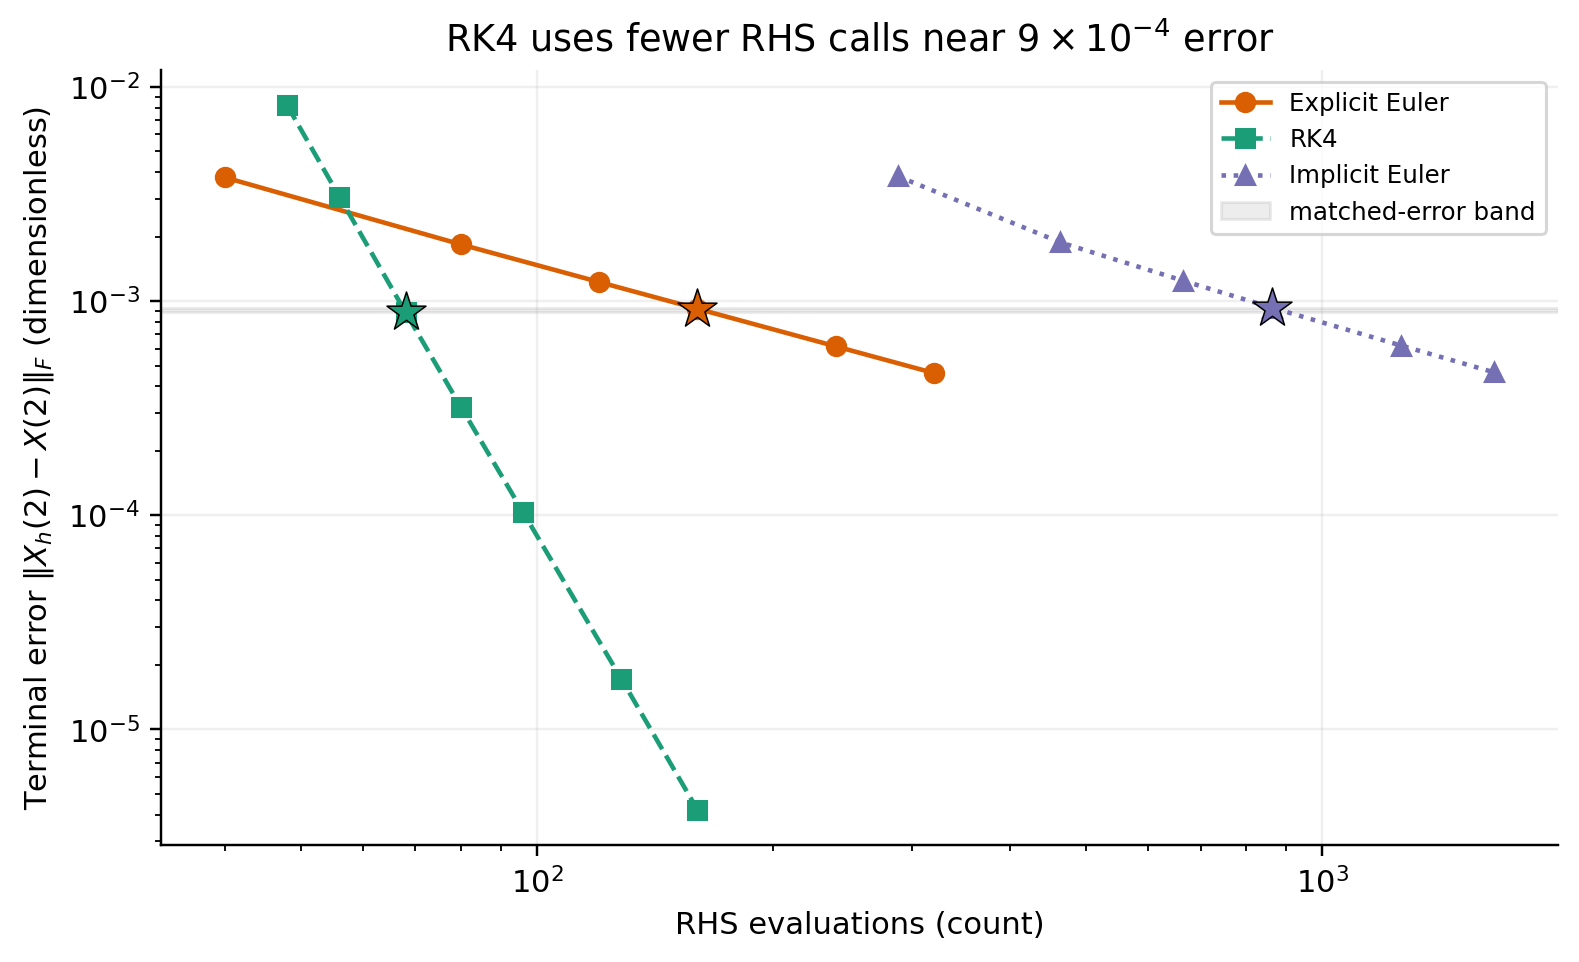
\includegraphics[width=0.86\textwidth]{cost_accuracy.png}
\caption{Achieved terminal full-matrix error versus counted RHS calls
over several fixed grids. Stars mark the three table entries with errors
near $9\times10^{-4}$; the grey band spans their actual errors. RK4
uses 68 RHS calls at this target, versus 160 and 862 for Explicit and
Implicit Euler. Jacobian and Newton costs are reported separately in
\texttt{cost\_accuracy.csv}, so RHS count is not wall-clock time.}
\label{fig:cost_accuracy}
\end{figure}

\paragraph{Rank-deficient initial state.}
Replacing the first initial singular value by zero and integrating
over $[0,8]$ with RK4 at $h=0.005$ leaves the smallest computed
singular value below $7.1\times10^{-15}$ throughout the stored path.
The two nonzero terminal singular values are approximately
$1.0000000500$ and $1.0000000276$; the final error against the
finite-time exact matrix is $3.86\times10^{-14}$.
The final orthogonality defect is approximately one, consistent with
a rank-two partial isometry rather than an orthogonal limit
(Fig.~\ref{fig:rank_deficient}).

\begin{figure}[htbp]
\centering
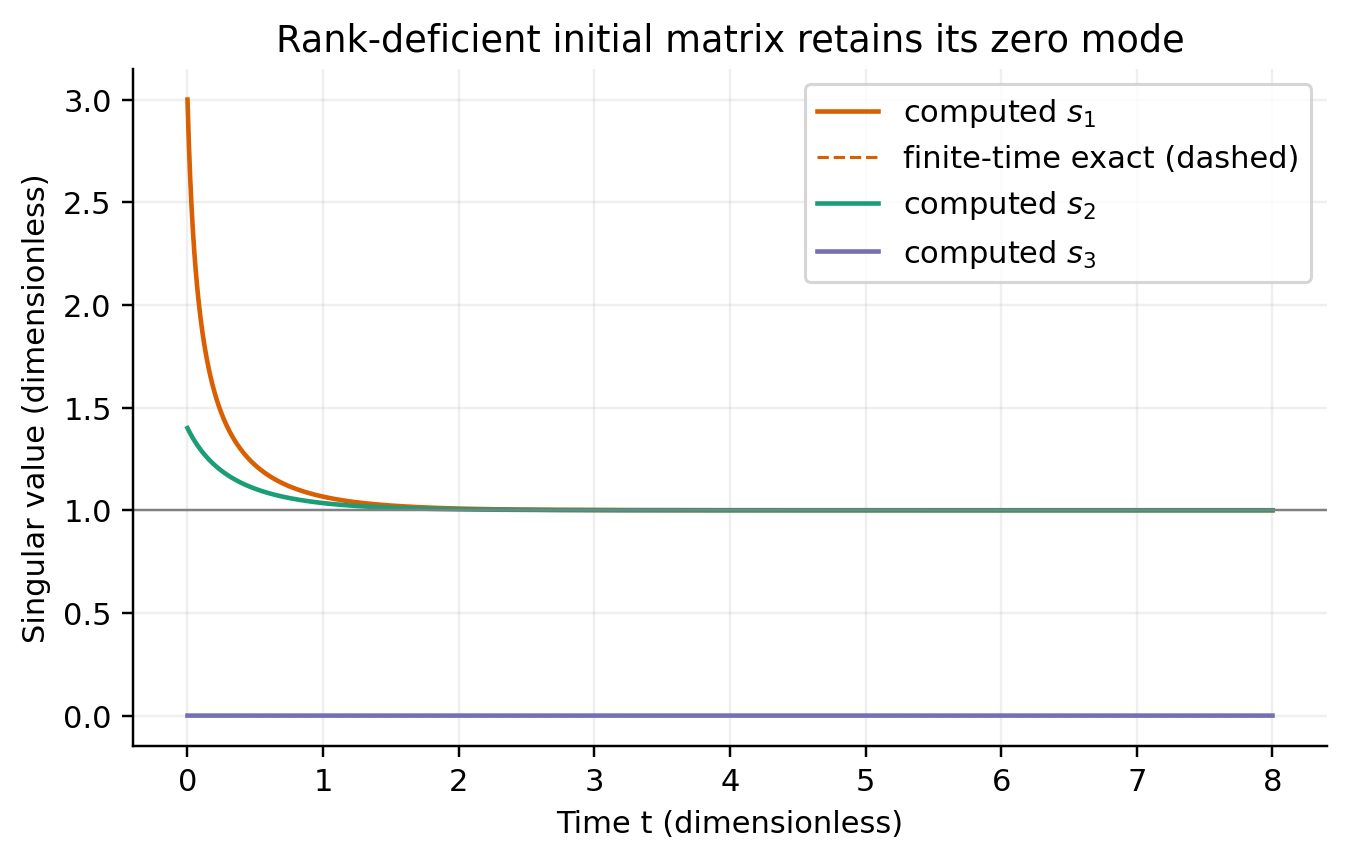
\includegraphics[width=0.78\textwidth]{rank_deficient.png}
\caption{The zero singular mode remains at round-off scale while the
other modes approach one, agreeing with the dashed exact SVD curves.
This distinguishes the partial-isometry limit from an orthogonal one.
Values are in
\texttt{rank\_deficient.csv}.}
\label{fig:rank_deficient}
\end{figure}


\subsection{Verification Coverage}
The runnable checks in \path{test/} comprise eleven test functions.
They check the model and full implicit-residual Jacobians by centred
finite differences, both complete eigenvalue spectra, the exact matrix
against tight-tolerance Radau, and a diagonal scalar sanity case.
All three methods are checked for fixed-grid order, genuinely varying
adaptive steps and accepted normalized estimated local errors at most
one. Their well-resolved trajectories are also checked for singular
values approaching one without crossing and non-increasing Lyapunov
energy. The rank-deficient check verifies the zero mode and convergence
toward the rank-two partial isometry. Independent subprocesses compare
both language versions for all three fixed and adaptive solvers.
The checks pass on the recorded environment.

The RK4 order test uses $N=640$ and $1280$, avoiding the finest
experiment grid whose error is nearer round-off scale. Passing these
checks supports the tested configurations; it does not turn the
local adaptive estimator into a universal global error bound.
The full numerical evidence and CSV interpretation are supplied in
Appendix~\ref{sec:appendix_c}.

\subsection{Limitations and Robustness}
The initial $h\lambda$ overlay is a frozen-Jacobian warning, not a
sufficient global nonlinear stability condition. An accepted
step-doubling estimate is likewise a local indicator rather than a
proof of global accuracy or stability. Large steps can destroy
monotonicity of $\Phi$ or cause an explicit run to fail; Newton may also
fail to find a decreasing candidate. The fixed-grid solver reports
such failures instead of changing the grid used to estimate order,
whereas the adaptive solver retries from the last accepted state.
Our matched-accuracy cost study counts RHS calls and reports Newton
work separately; a timing study would be needed to compare actual
runtime on a specified machine.

% ============================================================

\bigskip
\begin{thebibliography}{9}
\bibitem{hairer1993}
E. Hairer, S. P. N\o rsett, and G. Wanner,
\emph{Solving Ordinary Differential Equations I: Nonstiff Problems},
2nd ed., Springer, 1993. DOI: \href{https://doi.org/10.1007/978-3-540-78862-1}{10.1007/978-3-540-78862-1}.
\bibitem{higham1986}
N. J. Higham, ``Computing the Polar Decomposition---with Applications,''
\emph{SIAM Journal on Scientific and Statistical Computing}, 1986.
DOI: \href{https://doi.org/10.1137/0907079}{10.1137/0907079}.
\bibitem{virtanen2020}
P. Virtanen et al., ``SciPy 1.0: Fundamental Algorithms for Scientific Computing in Python,''
\emph{Nature Methods}, vol. 17, pp. 261--272, 2020.
DOI: \href{https://doi.org/10.1038/s41592-019-0686-2}{10.1038/s41592-019-0686-2}.
\end{thebibliography}

\clearpage
\appendix
\setcounter{section}{2}

\section{Supplementary Figures and Data}
\label{sec:appendix_c}

\subsection{Reproduction and Evidence Files}
This appendix documents the six CSV datasets and \path{summary.json}
used by the eight figures in Sections~2--4. Complete machine-readable
files are bundled in \path{report_v2/data/}; the corresponding submitted
images are in \path{report_v2/figures/}. The tables below are compact
readable extracts from those files. They preserve the full evidence
without replacing the CSV trajectories by rounded typeset values.

From the \path{Project1/} directory, run:
\begin{lstlisting}
python -m pip install -r requirements.txt
python -B code/run_all.py
python -B code_zh/run_all.py
python -B -m unittest discover -s test -v
\end{lstlisting}
The English run rebuilds project-level \path{figures/} and \path{data/};
the Chinese run uses \path{outputs_zh/}. In the recorded run, the two
languages give identical CSV/JSON contents and identical eight PNGs.
The regenerated English files also match this version's submitted
snapshots. PNGs are exported at 220 DPI.

All model quantities, time, and step lengths are dimensionless.
Evaluation and iteration fields are integer counts.
The model is deterministic, so no random seed is needed.
The stored singular values are in descending SVD order,
$s_1\geq s_2\geq s_3$; this ordering should not be confused with
the original diagonal input order $(0.2,1.4,3)$.

\subsection{Data-to-Figure Map}
\begin{table}[H]
\centering
\footnotesize
\begin{tabular}{@{}p{0.26\linewidth}rp{0.26\linewidth}p{0.32\linewidth}@{}}
\toprule
Evidence file & Rows & Associated figure(s) & Claim supported \\
\midrule
\path{convergence.csv} & 15 & \path{convergence.png} & Full-matrix errors, observed orders and fitted slopes. \\
\path{cost_accuracy.csv} & 19 & \path{cost_accuracy.png} & Achieved error and counted work at matched accuracy. \\
\path{stability_sweep.csv} & 39 & \path{stability_sweep.png} & Fast-direction amplification, geometry failures and failed runs. \\
\path{trajectory.csv} & 401 & \texttt{trajectory\_}\newline\texttt{diagnostics.png} & Singular values, energy, finite-time defect and Lyapunov residual. \\
\path{adaptive_steps.csv} & 3375 & \path{adaptive_steps.png} & Accepted time grid, varying step size and estimated local budget. \\
\path{rank_deficient.csv} & 1601 & \path{rank_deficient.png} & Numerical and exact singular values for the rank-two initial matrix. \\
\path{summary.json} & --- & \texttt{frozen\_spectrum.png},\newline \texttt{stability\_regions.png};\newline all experiment summaries & Settings, software versions, complete spectra, thresholds and aggregate diagnostics. \\
\bottomrule
\end{tabular}
\caption{Every numerical evidence file and the figure it supports.
Row counts exclude CSV headers. Stable filenames allow each reported
claim to be traced to the same version's full dataset.}
\label{tab:data_manifest}
\end{table}

\path{stability_regions.png} is evaluated directly from the three
analytic stability functions, with the initial spectrum overlaid.
It therefore has no separate sampled-trajectory CSV. Its amplification
formulas are in Section~2.3, the sampling grid and overlay step are in
\path{code/experiments.py}, and its spectrum is recorded in
\path{summary.json}. \path{frozen_spectrum.png} uses the same recorded
spectrum at $h=0.05$ and $0.10$.

\subsection{CSV Field Definitions and Missing Values}
\begingroup\raggedright
\paragraph{Convergence and cost.}
Both \field{convergence.csv} and \field{cost_accuracy.csv} contain
\field{method}, \field{n_steps}, \field{h},
\field{terminal_frobenius_error}, \field{rhs_evaluations},
\field{jacobian_evaluations}, and \field{newton_iterations}.
The terminal error is $\|X_h(2)-X_{\rm exact}(2)\|_F$.
The convergence file additionally stores \field{observed_order},
computed as $\log_2(E_h/E_{h/2})$; the first row of each method leaves
this field blank because no coarser comparison is available.
The cost file instead stores the Boolean \field{matched_point},
which identifies the starred comparison points. RHS counts include
nonlinear residual and line-search evaluations; Jacobian assembly,
factorization and plotting are not included in this cost measure.

\paragraph{Stability sweep.}
\field{stability_sweep.csv} contains \field{method}, \field{h},
\field{n_steps}, \field{one_step_fast_perturbation_amplification},
\field{one_step_energy_change}, \field{max_energy_increase},
\field{singular_value_crossing}, \field{terminal_exact_error}, and
\field{status}. Amplification is measured using an initial perturbation
of size $10^{-7}$ in the fastest singular-vector direction.
\field{status=diverged_or_failed} means the full run did not finish.
Blank or \field{nan} measurements in that row are unavailable quantities,
not zero error or zero amplification. The plotted curves use completed
runs; failed attempts remain in the CSV for inspection.

\paragraph{Resolved trajectory.}
\field{trajectory.csv} stores \field{t}, \field{s1}, \field{s2}, \field{s3},
\field{energy}, \field{exact_energy}, \field{orthogonality_defect},
\field{exact_orthogonality_defect}, and
\field{lyapunov_identity_residual_next_interval}.
The singular values, energy and defect refer to the row time.
The residual refers to the interval beginning at that row and is
plotted at its midpoint:
\[
D_n=\frac{\Phi(X_{n+1})-\Phi(X_n)}{t_{n+1}-t_n}
      +\left\|\bar X_n(I-\bar X_n^T\bar X_n)\right\|_F^2,
\qquad \bar X_n=\tfrac12(X_n+X_{n+1}).
\]
The final row has no following interval, so its residual is blank.
The figure shows $|D_n|$; the summary additionally reports the maximum
scaled residual with denominator $\max(1,|\dot\Phi(\bar X_n)|)$.
This scaled quantity is not a pure relative error.

\paragraph{Adaptive steps.}
\field{adaptive_steps.csv} stores \field{method}, \field{t_start},
\field{h}, and \field{normalized_local_error}. Each row represents an
accepted step from \field{t_start} to \field{t_start+h}.
The error is the normalized step-doubling estimate $E$ in Algorithm~2,
not the global terminal error. Accepted rows satisfy $E\leq1$.
The 3375 rows comprise 1680 Euler, 17 RK4 and 1678 Implicit Euler steps.
Rejected trial counts and independently measured terminal errors are
in \field{summary.json}. A final very short step may simply hit $t=2$.

\paragraph{Rank-deficient trajectory.}
\field{rank_deficient.csv} contains \field{t},
\field{s1}, \field{s2}, \field{s3}, and
\field{exact_s1}, \field{exact_s2}, \field{exact_s3}.
These are the numerical and finite-time exact sorted singular values
for $X_0=R(0.4)\operatorname{diag}(0,1.4,3)R(-0.7)^T$,
on $[0,8]$ with $h=0.005$.
The zero mode is the third column in the sorted numerical spectrum.

\par\endgroup
\subsection{Selected Numerical Evidence}
\begin{table}[H]
\centering
\small
\begin{tabular}{lrrrr}
\toprule
Method & $N$ & $h$ & $E_h(2)$ & Adjacent order \\
\midrule
Explicit Euler & 160 & 0.0125 & $9.2066\times10^{-4}$ & 0.9973 \\
Explicit Euler & 320 & 0.00625 & $4.6141\times10^{-4}$ & 0.9966 \\
RK4 & 640 & 0.003125 & $1.7123\times10^{-11}$ & 3.8039 \\
RK4 & 1280 & 0.0015625 & $1.1312\times10^{-12}$ & 3.9201 \\
RK4 & 2560 & 0.00078125 & $7.3968\times10^{-14}$ & 3.9348 \\
Implicit Euler & 160 & 0.0125 & $9.3194\times10^{-4}$ & 1.0114 \\
Implicit Euler & 320 & 0.00625 & $4.6429\times10^{-4}$ & 1.0052 \\
\bottomrule
\end{tabular}
\caption{Selected rows from \texttt{convergence.csv}. Adjacent orders
refer to the preceding coarser row in the complete dataset.
The finest RK4 error is near round-off scale; no plateau is inferred.}
\label{tab:appendix_order_rows}
\end{table}

\begin{table}[H]
\centering
\small
\begin{tabular}{lrrr}
\toprule
Method & Matched error & RHS calls & Jacobian/Newton updates \\
\midrule
Explicit Euler & $9.2066\times10^{-4}$ & 160 & $0/0$ \\
RK4 & $8.8502\times10^{-4}$ & 68 & $0/0$ \\
Implicit Euler & $9.3194\times10^{-4}$ & 862 & $351/351$ \\
\bottomrule
\end{tabular}
\caption{The \texttt{matched\_point=True} rows from
\texttt{cost\_accuracy.csv}. The largest error is approximately 5.3\%
above the smallest; this is a RHS-work comparison, not a runtime ranking.}
\end{table}

\begin{table}[H]
\centering
\small
\begin{tabular}{@{}p{0.61\linewidth}r@{}}
\toprule
Diagnostic from \path{summary.json} & Recorded value \\
\midrule
SVD/Radau terminal disagreement & $1.161\times10^{-13}$ \\
RK4 finite-time orthogonality defect & $0.305932824226$ \\
Exact finite-time orthogonality defect & $0.305932824210$ \\
Largest absolute midpoint Lyapunov residual & $0.239792$ \\
Largest scaled midpoint Lyapunov residual & $4.6936\times10^{-4}$ \\
Largest zero singular mode in rank-deficient run & $7.0899\times10^{-15}$ \\
Rank-deficient terminal exact-matrix error & $3.8613\times10^{-14}$ \\
Rank-deficient terminal orthogonality defect & $1.0000000000000064$ \\
\bottomrule
\end{tabular}
\caption{Checks supporting the finite-time, Lyapunov and rank-deficient
interpretations. The finite-time defect and discrete residual are not
expected to be zero.}
\end{table}

\subsection{JSON Contents and Version Traceability}
\path{summary.json} records the benchmark, interval and Newton residual
tolerance. It also records the software versions, convergence fit ranges
and slope standard errors, work counts at matched accuracy, Radau settings,
geometric checks, full initial and equilibrium spectra, local step-size
estimates, failed sweep runs, adaptive statistics and rank-deficient diagnostics.

The recorded environment is Python 3.12.4, NumPy 1.26.4,
SciPy 1.13.1 and Matplotlib 3.8.4. The initial full spectrum is
\[
(-26,-14.16,-8.64,-7.44,-5.76,-4.88,-1.28,-0.72,0.88),
\]
while the orthogonal-equilibrium spectrum has six $-2$ modes and
three zero modes, up to floating-point error. The positive initial
mode is physical growth, not a spurious instability.

\path{report_v2/manifest.json} records SHA-256 hashes of this report's
source, figures, data, verification record and code snapshot.
The Git tag \path{report-v2} identifies the matching whole-project
state. \path{report_v1/} remains a separate preserved snapshot,
with its corresponding project state identified by \path{report-v1}.
Further deliveries should use a new directory such as
\path{report_v3/} or \path{report_final/} and update the version index.

\end{document}
